% Note: use XeLaTeX for rendering
% !TEX encoding = UTF-8


\documentclass[twoside]{article}


%% Packages and their configuration
% Copyright 2022 Pierre S. Caboche. All rights reserved.

%% Packages and configuration

\usepackage{geometry}
\geometry{
	a4paper,
	total={170mm,257mm},
	left=35mm,
	right=35mm,
	top=30mm,
	bottom=30mm,
}


\usepackage{fontspec}
\setmainfont{DejaVu Serif} 
\setsansfont{DejaVu Sans} 

%% Use Sans-Serif by default
\renewcommand{\familydefault}{\sfdefault}


\usepackage{xeCJK}
\setCJKmainfont{Noto Serif JP}
\setCJKsansfont{Noto Sans JP}
\setCJKmonofont{Noto Sans Mono CJK JP}

\usepackage{xpinyin}


%% bibliography
\usepackage[authoryear]{natbib}

%% index
\usepackage{imakeidx}
\makeindex


\usepackage{xcolor}
\usepackage{graphicx}


\usepackage{titleps}
\usepackage{xstring}
\newcommand{\currentPart}{}

\newcommand{\formatPartTitleDefault}{
	\textbf{\IfStrEq{\thepart}{}{}{Part \thepart\ ---  }\currentPart}
}

\newcommand{\formatPartTitle}{\formatPartTitleDefault}

\newcommand{\copyrightNotice}{\color{gray}{\emph{\textcopyright\ 2022 Pierre S. Caboche. All rights reserved.}}}

\newpagestyle{main}{
	\sethead
	% even
	[\formatPartTitle]
	[]
	[]
	% odd
	{}
	{}
	{\formatPartTitle}
	
	\setfoot
	% even
	[\textbf{\thepage\ \color{lightgray}{|}}]
	[]
	[\copyrightNotice]
	% odd
	{\copyrightNotice}
	{}
	{\textbf{\color{lightgray}{|} \color{black}{\thepage} }} 
	
	\headrule
	%\footrule
}
\pagestyle{main}

\widenhead[25pt][25pt]{25pt}{25pt}



\usepackage{listings}
\lstset{
	basicstyle=\fontsize{9}{9}\selectfont\ttfamily
	,frame=lines
	,tabsize=2
	,keywordstyle=\bfseries%\itshape,
	,commentstyle=\itshape\color{teal}
	,stringstyle=\color{magenta}
	,breaklines=true,
	,postbreak=\mbox{\textcolor{red}{$\hookrightarrow$}\space}
}



\usepackage{hyperref}
\usepackage{longtable}
\usepackage[super]{nth}



\widowpenalties 1 10000
\raggedbottom

\setlength{\parindent}{0pt}



%% Custom macros
% Copyright 2022 Pierre S. Caboche. All rights reserved.

\usepackage{mdframed}
\mdfsetup{
	%innertopmargin=10pt,
	frametitleaboveskip=-\ht\strutbox,
	frametitlealignment=\center
}


\newcommand{\note}[1]{
	\mdfsetup{
		middlelinewidth=2pt,
		backgroundcolor=yellow!10
	}
	\begin{mdframed}#1\end{mdframed}
	\mdfsetup{
		backgroundcolor=white
	}
}


\newcommand{\cmd}[1]{\lstinline|#1|}


\newcommand{\python}{Python}
\newcommand{\awk}{AWK}
\newcommand{\perl}{Perl}
\newcommand{\julia}{Julia}
\newcommand{\gawk}{\texttt{gawk}}
\newcommand{\mawk}{\texttt{mawk}}
\newcommand{\sed}{\texttt{sed}}
\newcommand{\grep}{\texttt{grep}}

\newcommand{\stdin}{\texttt{stdin}}
\newcommand{\stdout}{\texttt{stdout}}
\newcommand{\stderr}{\texttt{stderr}}

\newcommand{\mysqldump}{\texttt{mysqldump}}
\newcommand{\cat}{\texttt{cat}}
\newcommand{\pv}{\texttt{pv}}
\newcommand{\shell}{\texttt{shell}}

\newcommand{\Unix}{UNIX\textregistered}
\newcommand{\Intel}{Intel\textregistered}
\newcommand{\Core}{Core\texttrademark}




%% Our function for adding furigana
% This source code is under the BSD License
% Copyright 2022 Pierre S. Caboche

\usepackage{ruby,tikz}
\newcommand{\furi}[1]{\foreach \kanji/\furigana in {#1}{\ruby{\kanji}{\furigana\vphantom{あ}}}}


%% Configuration for "ruby" package (loaded by 'files/furi')
\renewcommand{\rubysize}{0.4}     % default:  0.4
\newcommand{\defaultrubysep}{0ex} % default: -0.5ex
\renewcommand{\rubysep}{\defaultrubysep}




%opening
\title{
Solr and ElasticSearch:
\\ 
index, faceting, and 
\\
analysing the lyrics of Japanese songs}

\author{Pierre S. Caboche ( \furi{南瓜/カボチャ}ピエール )}


% Custom format to indicate revision date (when needed)
\date{
	September 12, 2022 \\
%	\medskip 
%	\footnotesize \emph{Revised: \today}
}


\begin{document}

\maketitle



\begin{abstract}

\bigskip

このドキュメントは、日本語の歌詞の\furi{単語/たんご,の/,使用状況/しようじょうきょう,を/,統計的/とうけいてき,に/,分析/ぶんせき,が/,含/ふく}まれています。 \furi{結果/けっか}は「Part \ref{analysing-lyrics}」(\pageref*{analysing-lyrics}ページから\pageref*{analysing-lyrics-end}ページまで)に示されています。

This document contains a statistical analysis of word usage in the lyrics of Japanese songs. The results are shown in part \ref{analysing-lyrics} (pages \pageref*{analysing-lyrics} to \pageref*{analysing-lyrics-end}). \\
	
\bigskip
	

This article's content is divided as follows:
\begin{itemize}
	\item \textasciitilde 20\%: learning about Solr, full-text search, faceting, and associated concepts
	\item \textasciitilde 10\%: learning how to use those concepts in ElasticSearch, and showing some differences between ElasticSearch and Solr
	\item \textasciitilde 70\%: applying what we learned to analyse the lyrics of Japanese songs, in terms of vocabulary used
\end{itemize}	

\bigskip

In other words, we will give you a quick introduction to Solr and ElasticSearch, then the bulk of this article will be about seeing the tools in action on some interesting, real-world example.

Our goal with this example, will be to answer questions like: \emph{``What kind of words are usually used by different bands / songwriters ?"} (to identify trending words, understand the writing styles of different artists, and find similarities between bands). \\

For this, we will use \emph{Solr} (an enterprise-search platform based on \emph{Apache Lucene}), and try to replicate the results on the increasingly popular \emph{ElasticSearch}.

All the documents to index are in Japanese, which will allow us to learn about \emph{morphologic analysers}, \emph{lemmatisation}, and the challenges associated with indexing texts in different languages. \\

\bigskip

Therefore, this article may appeal to different audiences:
\begin{itemize}
	\item software developers who want to learn about \emph{Solr}, \emph{ElasticSearch}, full-text search, \emph{faceting}, \emph{aggregations}, etc.
	
	\item people interested in Japanese music
	
	\item people interested in learning Japanese
\end{itemize}


\bigskip


\end{abstract}

\newpage


%%% Intro


%%% TOC
\newpage
\renewcommand{\currentPart}{Table of Contents}

\addtocontents{toc}{\setcounter{tocdepth}{3}}
\setcounter{tocdepth}{3}
\tableofcontents

 
%%% Article body

\newpage
% Copyright 2022 Pierre S. Caboche. All rights reserved.

\renewcommand{\currentPart}{First words}
\part{\currentPart}


\section{Introduction}

I was experimenting with Solr and ElasticSearch when I discovered that, in Solr, performing some \faceting\ on a field of type \emph{text} returned some statistics on word usage. \\

Normally, \faceting\ is used to provide some statistic information about the result of a query (e.g. \emph{document count, sum, min, max, average, percentile}\dots). Faceting is usually applied on fields of type \emph{string(s)} (e.g. to group by tags, categories, etc.), or by defining ranges on some numeric values. ElasticSearch takes the concept of \faceting\ even further with its \aggregations\ (section \ref{faceting-and-aggregation}).


Performing \faceting\ on a field of type \emph{text} is not common. In fact, this is not enabled by default in ElasticSearch, for a question of performance (sections~\ref{create-es-core} and~\ref{aggregation-termsVectors}).
\\


Seeing the document counts for different words gave me an idea: to use this feature for analysing the writing style of different artists. Also, is the \MLT\ facility to find similar \oe uvres (section~\ref{mlt}).
\\

In my spare time, I listen to a lot of Japanese music from a variety of artists. I study the lyrics, look for the words that I do not know, practice at the \emph{karaoke}.
This is why I decided to perform the text analysis on Japanese songs. I also had access to a rather large collection of lyrics, parts of which I could use as a dataset. \\

This case study is interesting because it will allow us to learn about :
\begin{itemize}
	\item full-text search, indexing, morphologic analysers, etc.
	
	\item managing texts in different languages
	
	\item \faceting, \aggregation, which are essential to providing statistical data on a query result-set
\end{itemize}



If you like Japanese music (like I do), this article may give you some insights about the word usage of your favourite artists. \\


In this article, we will do the following:
\begin{itemize}
	\item introduce the tools (Solr and ElastiscSearch)
	
	\item introduce the general concepts which will be used in both Solr and ElastiscSearch (Part~\ref{part - A bit of theory})
	
	\item present our solution, starting with all the Solr-specific implementation details  (Parts~\ref{part- Quick introduction to Solr} and~\ref{part - Running Solr})
	
	\item show some of the considerations that come with handling different languages (Part~\ref{part - Challenges})
	
	\item use Solr, run the analysis, display the results (Part~\ref{analysing-lyrics})
	
	\item try to replicate the analysis with ElasticSearch (as a proof-of-concept). Show the differences with Solr (Part~\ref{part - ElasticSearch})
	
	\item compare the two solutions, in terms of: features, implementation, etc. (Part~\ref{part - Final words})
\end{itemize}

\bigskip


\newpage



\section{The tools}

Below is a quick introduction to the technologies we are going to use in this article:

\subsection{Lucene}

Apache Lucene is a free and open-source search engine software library, originally written in Java. \\

Lucene is the technology that powers both Solr and ElasticSearch. \\

Lucene is supported by the Apache Software Foundation and is released under the Apache Software License. It has been ported to a number of languages besides Java.



\subsection{Solr}

Solr (pronounced "solar") is an open-source enterprise-search platform, written in Java and powered by Lucene. It is developed by the Apache Software Foundation. \\

Solr provides features such as: full-text search, hit highlighting, faceted search, and more. Interacting with Solr can be done through an HTTP web interface and schema-free JSON documents. \\

Solr servers can run in a cluster, in which indexes are replicated. This improves scalability, fault tolerance, and allows for search to be distributed between servers.



\subsection{ElasticSearch}

ElasticSearch is an extremely popular, proprietary enterprise-search platform, written in Java and powered by Lucene. It is developed by the company Elastic~NV. \\

Much like Solr, it provides full-text search, hit highlighting, aggregations\dots\ Interaction can be done through an HTTP web interface and schema-free JSON documents; ElasticSearch supports dynamic clustering, index replication, to achieve scalability, fault tolerance, and allow for  distributed search. \\

The ElasticSearch ecosystem (a.k.a. the \emph{``Elastic Stack"}) also includes: Kibana (for data visualisation, Machine Learning, Alerts\dots), Logstash (for data collection and integration). Some features (e.g. Machine Learning) are only accessible with the appropriate subscription level. \\


\bigskip

\newpage

\section{Prerequisites}

\emph{Part~``\longref{analysing-lyrics}"} does not require any technical knowledge, as it shows the results of our statistical analysis of word usage in Japanese songs. \\

For the rest of this document (which explains how we arrived at the results in Part~\ref{analysing-lyrics}), some technical knowledge is necessary. \\

Below is the list of prerequisites to follow along the technical parts of this document:


\begin{itemize}
	\item no knowledge of \emph{Solr} or \emph{ElasticSearch} is required to follow this article. We will explain the core principles as needed
	
	\item for simplicity and ease of use, we will use \emph{Docker} to run Solr and ElasticSearch in a virtual, containerised environment.
	
	You need to have both \textbf{Docker} and \textbf{docker-compose} installed and ready to run on your system
	
	\item we use \textbf{Linux scripts} to run how environments. 
	
	Some knowledge of \emph{shell}, \emph{AWK}, or \emph{sed} will help you understand how the scripts work, but is not strictly necessary.
	
	It should be possible to run the scripts on Windows, using WSL 2 (Windows Subsystem for Linux 2), but please bear in mind that \emph{localhost} refers to the Linux virtual machine running on WSL 2. Accessing a service running on the Windows host from the WSL 2 Linux machine is a bit tricky\dots
	
	\item a basic understanding of \textbf{Web Services} is an advantage, as this is how we usually interact with Solr and ElasticSearch
	
	\item a basic understanding of \textbf{JSON} is necessary, as this is the format that we will use to exchange data with Solr and ElasticSearch (both the documents in input, and the query responses are in JSON format)
\end{itemize}



\newpage

\section{About the dataset\dots}

Normally when I write an article, I try to provide the reader with all the necessary information they would need to reproduce the experiments, as well as explore the data on their own, perform their own experimentations and come to their own conclusion. \\

However, for this this article, this is not possible\dots\ because of copyright laws. \\

Songs (both the music and the lyrics) are subject to copyright laws. \\



A copyright is a form of intellectual property protection. It covers \emph{original works} and is generated \emph{automatically} upon creation of said work.
Items that can be copyrighted include: poetry, novels, art, movies, research\footnote{which includes this paper}, songs\dots\ \\

Individual words cannot be copyrighted. Words can be subject to trademark, a different kind of intellectual property protection which requires registration (and therefore is not automatic). \\


For this reason, \emph{I cannot publish the dataset that this study is based on}, because the lyrics it contains are subject to copyright (despite the dataset being assembled from publicly-available information). \\

I can, however, provide you with the results of this study (some statistical data about word usage). \emph{It is impossible to reconstruct the original lyrics based on the results of this study.}

\bigskip
\bigskip




\newpage
\section{General Information}

This document was first published at: \\
\mbox{} \hfill \url{https://pcaboche.github.io} 

\subsection{Legal}
\input{"READ_ME_(LEGAL).txt"}


\bigskip
\bigskip

\section{Conventions}

\subsection{Name order}

Japanese names consist of a family name (surname), followed by a given name, in that order. \\

When transcribing Japanese names into English, the policy ever since the Meiji era was to follow the English way of ordering names (i.e. first name first, family name last). However, in recent years this policy is being challenged, and Japanese names now tend to follow Japanese name order convention, even when transcribed in English. \\

In this article, we follow the Japanese convention for ordering name (i.e. family name first) \emph{except} when the artist chose a different convention as their stage name (e.g. \emph{Kaneko Ayano}). \\






\newpage
% Copyright 2022 Pierre S. Caboche. All rights reserved.


\renewcommand{\currentPart}{A bit of theory}
\part{\currentPart} \label{part - A bit of theory}

This part will us a quick overview of the concepts that make our text analysis possible in both Solr, and ElasticSearch.


\section{Lemmatisation} \label{lemmatisation}

\begin{displayquote}
Lemmatisation (or lemmatization) in linguistics is the process of grouping together the inflected forms of a word so they can be analysed as a single item, identified by the word's lemma, or dictionary form. \\
\phantom{.} \hfill -- \url{https://en.wikipedia.org/wiki/Lemmatisation}
\end{displayquote}
\bigskip

For example in English, the verb ``to be" can take the following forms (inflexions): \emph{to be, be, am, are, is, 'm, 're, 's, was, were, isn't, aren't, wasn't, weren't, ain't\dots} \\

Japanese also has inflexions (for verbs and i-adjectives), for example the verb 会う (au - ``to meet")\footnote{do not to confuse the verb 会う (au - ``to meet") with 合う (au - \emph{"to match"}). Same pronunciation, similar \emph{kanji}, different verbs\dots} can conjugate into: 会います (aimasu), 会わない (awanai), 会って (atte), 会った (atta), 会おう (aou), 会え(ae), 会うな (auna), 会える (aeru), 合われる (awareru)\dots\\

On top of having inflections as shown above, Japanese also features \emph{agglutinations}, which allows to change the meaning of verbs and i-adjectives by stringing together some \emph{morphemes} (to make the negative form, past form, passive form, etc). \\

For example, the verb 会う (au - \emph{"to meet"}) can conjugate into from 会います (aimasu - \emph{``(is) meeting"}) from which we derive the adjective\footnote{you read that right: the verb turned into an i-adjective} aitai (会いたい - \emph{``want to meet"}) which can then turn into, for example:
\begin{itemize}
	\item aitakunai (会いたくない) - \emph{``don't want to meet"}
	\item aitakatta (会いたかった) - \emph{``wanted to meet"}
	\item aitakunakatta (会いたくなかった) - \emph{``didn't want to meet"}
	\item aitakunakattakutemo (会いたくなかったくても) - \emph{``whether (X) wanted to meet or not"}
\end{itemize}

%All of the forms above derive from the verb 会う (au - \emph{"to meet"}), not to be confused with the verb 合う (au - \emph{"to match"}). \\

All those forms derive from the same \emph{lexeme} (by \emph{inflection}, \emph{agglutination}, or both). \\

A \emph{lemma} is a particular inflection that is chosen to represent words belonging to the same \emph{lexeme}. 

This is often referred to as the ``dictionary form", ``canonical form", or ``citation form". By convention, for verbs it's the infinitive form which is chosen as the ``canonical form" (in this example: 会う ).\\

During the \emph{lemmatisation} process, words in a text will be replaced by their canonical form. 
These will then be used as \emph{tokens} in the \emph{tokenisation} process (section~\ref{tokenisation}). \\




\section{Morphologic analysers} \label{morphologic-analysers}


\begin{displayquote}
\emph{``Morphology, in linguistics, is the study of the forms of words, and the ways in which words are related to other words of the same language."}  \\
\phantom{.} \hfill -- \url{https://cowgill.ling.yale.edu/sra/morphology_ecs.ht}
\end{displayquote}
\bigskip

A \emph{morphologic analyser} is a piece of software which will take a text in a certain language, analyse this text, and extract the structure of this text. \\

From there, it is possible to extract a list of \emph{lexemes} (section \ref{lemmatisation}), together with some extra information (e.g. lexeme position, offset), which can be used for the \emph{tokenisation} process (section \ref{tokenisation}). \\


\subsection{The kuromoji analyser}  \label{kuromoji}

In Lucene (the project which powers both Solr and Elasticsearch), the analysis of texts in Japanese is done using \kuromoji, an open source Japanese morphological analyser written in Java. \\

Kuromoji can be used on its own. \\

According to its website (see below), \kuromoji\ has been donated to the Apache Software Foundation. \\

Website: \hfill \url{https://www.atilika.org} \hfill \hphantom{.} \\


\section{Tokenisation} \label{tokenisation}

\emph{Tokenisation} (or \emph{tokenization}) is the process of breaking down some input (e.g. a piece of text) into small units called \emph{tokens}. \\ 

Such tokens are an essential part of indexing (for Solr, ElasticSearch), or Natural Language Processing (NLP). \\

For text, a \emph{morphologic analyser} (section \ref{morphologic-analysers}) for the appropriate language is used to extract the tokens which will be used for indexing. \\

Custom \emph{tokenisers} can also be written to extract important information from a file in a specific format. \\


\section{tf–idf} \label{tf–idf}


\begin{displayquote}
\emph{``In information retrieval, \emph{tf–idf}, short for \emph{term frequency–inverse document frequency}, is a numerical statistic that is intended to reflect how important a word is to a document in a collection or corpus."}  \\
\phantom{.} \hfill -- \url{https://en.wikipedia.org/wiki/Tf%E2%80%93idf}
\end{displayquote}
\bigskip

In other words, \emph{tf–idf} is a measure of \emph{``how often a \emph{term} appears in a document \emph{(term frequency)} relative to how often it appears in general, across all documents \emph{(inverse document frequency)}?"}

\emph{tf–idf} is used to measure the \emph{relevance} of a document given a search query. \\

\emph{tf–idf} is also used to find documents with similar word-usage, as we will see in section \emph{\longref{mlt}}.

\bigskip

There are different ways to weigh both the \emph{term frequency} and \emph{inverse document frequency}. For more information on \emph{tf–idf}, see: \\
\phantom{.} \hfill
\url{https://en.wikipedia.org/wiki/Tf%E2%80%93idf}





\section{TermsVector}

\emph{tf–idf} term vectors are a data-structure which is used to represent text documents, with the intent of performing text mining and machine learning operations. \\

\emph{termVector}s contain information about terms, such as: term (lexeme), frequency, position, start offset, end offset. \\

We will be able to visualise the content of \emph{termVector} in ElasticSearch in sections~\ref{es-testing-kuromoji} and \ref{es-viewing-termsVector}.


\bigskip


\section{Faceting and Aggregations} \label{faceting-and-aggregation}


\emph{Aggregations} (an extension of \faceting), is a very important concept in Solr and ElasticSearch. Our whole statistical study relies on such concepts. \\

\medskip

A \emph{facet} takes a set of documents as input (as returned by a query) and outputs a summary, based on document counts (e.g. number of documents that fall into a certain category / are marked with a certain tag). \\



\emph{Aggregations} takes this concept a lot further. As mentioned in the documentation:




\begin{displayquote}
	\emph{``Elasticsearch organizes aggregations into three categories:}

	\begin{itemize}
		\item \emph{\emph{Metric} aggregations that calculate metrics, such as a sum or average, from field values.
		\item \emph{Bucket} aggregations that group documents into buckets, also called bins, based on field values, ranges, or other criteria.
		\item \emph{Pipeline} aggregations that take input from other aggregations instead of documents or fields.}
	\end{itemize}" \newline
	--- \url{https://www.elastic.co/guide/en/elasticsearch/reference/current/search-aggregations.html}
\end{displayquote}

\bigskip

ElasticSearch uses the term \aggregation\ (and all their features). \\

Solr uses the term \faceting, and has more limited capabilities (but are easier to use, and are enough for our use-case). \\





\newpage
% Copyright 2022 Pierre S. Caboche. All rights reserved.

\renewcommand{\currentPart}{Quick introduction to Solr}
\part{\currentPart}  \label{part- Quick introduction to Solr}


\section{Overview of Solr}

Solr is an enterprise-search platform, which means it is designed to index data and documents from various sources (e.g. databases, file systems, e-mails. etc.) \\


In Solr, information is organised as such:

\begin{itemize}
	\item \texttt{Core} \hfill
	
	A \emph{core} is a collection of \emph{documents}
	
	\item \texttt{Document} \hfill
		
	Information that needs to be queried together is stored in the same \emph{document}. Documents are made up of \emph{fields}.
	
	Each document is identified with an \texttt{id} field, which must be unique, but can be automatically generated (section \ref{id-field}).
	
	\item \texttt{Field} \hfill
	
	A field is a piece of information that can be queried.
	
	Fields can be defined explicitly (section \ref{defining-fields}), or dynamically (section \ref{dynamic-fields}).
	
	Sometimes the same information needs to be indexed, stored, and queried in different ways. (\longref{copy-fields})
\end{itemize}


Text fields can be analysed, and the index may be stored (with different options such as: terms positions, frequency, etc). Different languages require specific analysers. The analyser for Japanese is called \kuromoji\ (section \ref{kuromoji}).






\section{The \texttt{id} field}   \label{id-field}

In Solr, every document must have a field named \texttt{id}, of type \texttt{string}, which is used to uniquely identify a document. \\

Here are a few things to bear in mind when choosing an \texttt{id}:

\begin{itemize}
	\item avoid using numeric identifiers (i.e. 1, 2, 3...) \\
	
	If your \texttt{id} is exposed to the outside world, it would then be easy for an outsider to retrieve the content of your documents just by going through different numeric values \\
	
	
	\item use characters that can be easily passed in a URL \\

	Most of the time we will need to interact with our documents through a Web API, and the id needs to be passed as part of the URL. \\
		
	If your \texttt{id} is not "URL-friendly" then you'll need to encode it, one way or another, to be passed in a URL. Solutions include:
	
	\begin{itemize}
		\item \emph{URL-encoding}
		
		Special characters are escaped to be used in a URL. \\
		
		\item \emph{base64}
	
		allows to convert some binary data as input into a string of 64 different characters (hence the name). The resulting string is around 33 to 37\% longer than the original binary data but has a number of applications, especially on the web. \\
		
		The \emph{base64} \texttt{id} can be either generated from a random string, or derived from the data itself. Platforms like YouTube use \emph{base64} for their \texttt{id}s.
	\end{itemize}
	

	
\end{itemize}



\bigskip


\section{Fields}

\subsection{Defining Fields} \label{defining-fields}

Each field must have at least:
\begin{itemize}
	\item a \emph{name}
	\item a \emph{type}
\end{itemize}


A field \emph{may} also have (optional):
\begin{itemize}
	\item a \emph{default value}
	
	\item \emph{Field Type Override Properties} which define how the field might be stored, indexed, and other properties
\end{itemize}


\subsubsection*{Field Types}

Below are some examples of field types we might encounter:

\begin{longtable}{| p{2.5cm} p{7.5cm} p{3.5cm} |}
	\hline
	Type
	&
	Description 
	& 
	
	Elasticsearch's \newline
	closest 
	equivalent 	
	\\
	\hline
	& & \\
	\endhead
	
	\hline
	\endfoot
	
	\texttt{string}
	&
	String (UTF-8 encoded string or Unicode).
	Has a hard limit of slightly less than 32K.
	Intended for small fields and are not tokenised or
	analysed.
	
	Examples: ID, email, hostname, postal code, tags...
	Useful for aggregations (e.g. by tag).
	
	& 
	\texttt{keyword}
	\\
	
	
	\texttt{text\_general}
	&
	Textual information.
	&
	\texttt{text}, \newline
	using the standard analyser \newline
	\\
	
	
	\texttt{text\_en}
	&
	Textual information. \newline
	Makes use of the analyser for the English language.
	&
	\texttt{text}, \newline
	using the english analyser \newline
	\\
	
	
	\texttt{text\_ja}
	&
	Textual information. \newline
	Makes use of the \kuromoji\ analyser (section~\ref{kuromoji}) for the Japanese language.
	&
	\texttt{text}, \newline
	using the \kuromoji\ analyser (plugin) \newline
	\\
	
	
	\texttt{text\_...}
	&
	Other \texttt{text} types are available, using different
	analysers.
	&
	\texttt{text}, \newline
	using the 
	analyser of your choice \newline
	\\
	
	
	\texttt{pdate}
	&
	Date. \newline
	Represents a point in time with milliseconddate ,
	precision.  \newline
	Example: Album release date. \newline
	&
	\texttt{date}, \newline
	\texttt{date\_nanos}
	\\
	
\end{longtable}


\bigskip




\subsubsection*{Field Type Override Properties}


\begin{longtable}{| p{2.5cm} p{1.5cm} p{9cm} |}
	\hline
	Property
	&
	Implicit default
	&
	Description
	\\
	\hline
	& & \\
	\endhead
	
	\hline
	\endfoot

	\texttt{required}
	&
	\texttt{false}
	&
	Instructs Solr to reject any attempts to add a document which
	does not have a value for this field. This property defaults to
	false. \newline
	\\
	
	
	\texttt{multiValued}
	&
	\texttt{false}
	&
	If true, indicates that a single document might contain multiple
	values for this field type. \newline
	\\
	
	
	\texttt{stored}
	&
	\texttt{true}
	&
	If true, the actual value of the field can be retrieved by queries. \newline
	\\
	
	\texttt{indexed}
	&
	\texttt{true}
	&
	If true, the value of the field can be used in queries to retrieve
	matching documents. \newline
	\\
	
	
	\texttt{docValues}
	&
	\texttt{false}
	&
	If true, the value of the field will be put in a column-oriented DocValues structure (a way of recording field values internally that is more efficient for some purposes, such as sorting and faceting, than traditional indexing). \newline
	
	DocValues are only available for specific field types (string, boolean, numeric, date...) \newline
	\\
	
	
	\texttt{uninvertible}
	&
	\texttt{false}
	&
	\emph{Defaults to true for historical reasons, but users are strongly encouraged to set this to false for stability and use
	\texttt{"docValues":"true"} as needed.} \newline
	\newline
	If true, indicates that an \newline
	\texttt{"indexed":"true", "docValues":"false"} field can be \newline ``un-inverted" at query time to \emph{build up large in memory data structure} to serve in place of DocValues. \newline
	\\
	
	
	
	\texttt{termVectors, termPositions, termOffsets, termPayloads}
	&
	\newline
	\texttt{false}
	&
	These options instruct Solr to maintain full \texttt{term vectors} for
	each document, optionally including \texttt{position}, \texttt{offset} and	\texttt{payload} information for each term occurrence in those vectors. \newline
	\newline
	These can be used to accelerate highlighting and other ancillary functionality, but impose a substantial cost in terms of index size. \newline
	\\
\end{longtable}

\bigskip

For more information about fields in Solr: \\

\url{https://solr.apache.org/guide/solr/latest/indexing-guide/fields.html} \\


\href{https://solr.apache.org/guide/solr/latest/indexing-guide/field-types-included-with-solr.html}{\texttt{https://solr.apache.org/guide/solr/latest/indexing-guide/field-types-included-\newline
with-solr.html}} \\

\url{https://solr.apache.org/guide/solr/latest/indexing-guide/docvalues.html}



\bigskip
\bigskip
\bigskip

\subsection{Dynamic fields} \label{dynamic-fields}

A dynamic field is like a field that has a name with a wildcard in it. \\

When indexing a document, Solr will try to match field names with:
\begin{enumerate}
	\item explicitly defined fields
	\item dynamic fields
\end{enumerate}

\bigskip

By using dynamic fields, it becomes easy to add new fields of a certain types by following some naming conventions. \\

For example (the following are defined by default in Solr):

\begin{longtable}{l p{12.5cm}}
	\cmd{*\_str} & Field of type \cmd{strings} (DocValues, Multivalued, Sort Missing Last). \\
	& Used for storing lists of \cmd{keywords} (tags, categories). \\
	& \\
	\cmd{*\_txt\_ja} & Filed of type \cmd{text\_ja} (Indexed, Tokenized, Stored, UnInvertible) \\
\end{longtable}

\bigskip


Think of dynamic fields as \emph{``convention over configuration"}. \\


\newpage

\subsubsection{Explicit vs. Dynamic fields} \label{explicit-vs-dynamic}

The advantage of explicit fields is, you can describe the exact structure of your documents, and also specify which fields are required (and that requirement will be enforced). 

The main drawback is, specifying fields explicitly is tedious, there are lots of options, and any change in the schema can be costly (there is a need to re-index documents for newly specified fields to be taken into account).
\\




The advantage of dynamic fields is, you can easily add new fields ``on the fly" without modifying the schema. 

The main drawback of dynamic fields is, you need to follow certain conventions, which forces you to rename some fields from your original JSON object (and adapt your queries to match this naming convention too). \\

In our example, we will use dynamic fields a lot. We find it easier to rename fields so that they match the desired convention, rather that declaring each field separately. \\

Also, by following a convention it is easier to remember the purpose of a given field, just by looking at its name (e.g. \cmd{*\_str} fields are for \emph{tags} and other lists of predefined values, while \cmd{*\_txt\_ja} fields have been indexed using the Japanese analyser). \\


\bigskip

\subsection{Copy fields} \label{copy-fields}

It is possible to specify that, on indexing, some values must be copied from one field to another. \\

This allows:
\begin{itemize}
	\item to have different representations of the same data
	\item to concatenate different pieces of information (e.g. title, author, etc.) into one field that is easy to query (instead of writing complex queries which will impact performance)
\end{itemize}

\bigskip


\newpage

\section{Defining a schema}

A schema allows you to explicitly define:

\begin{itemize}
	\item what fields will be used (names and types)
	\item which fields are required
	\item how each field is indexed
	\item which fields need to be copied from one another (\cmd{copyField})
\end{itemize}

It is also possible to define new Dynamic Fields.

\bigskip


A schema can be specified either:
\begin{itemize}
	\item in the \cmd{schema.xml} file
	\item through the \href{https://solr.apache.org/guide/solr/latest/indexing-guide/schema-api.html}{Solr Schema API}
\end{itemize}

\bigskip

It is easier to interact with the Solr Schema API than with files. That being said, we find it even easier to rely dynamic fields, as explained in sections \ref{dynamic-fields} and \ref{explicit-vs-dynamic}.





\newpage
% Copyright 2022 Pierre S. Caboche. All rights reserved.


\renewcommand{\currentPart}{Challenges}
\part{\currentPart}  \label{part - Challenges}

Now that we know more about Solr and some of the concepts behind it, we will talk about the things to consider when dealing with texts in multiple languages. We will also see some of the challenges posed by a language like Japanese.


\section{Challenges when indexing different languages}

For our case study we want to focus on analysing songs in Japanese, but it is possible to extend this model to other languages. \\

When dealing with information in different languages, it is necessary to use separate morphological analysers. This is because each analyser is specialised to identify lexemes in one language. This also means having to store information in separate fields. \\

There are mainly two ways to handle this problem. \\

The first solution is to have \emph{one field per language}, as follows:
\begin{itemize}
	\item declare one field per language, using the appropriate type (using the analyser for that language)
	
	\item if necessary, use ``copy fields" (section \ref{copy-fields}) to copy the content of all the language-specific fields, to a field that uses the standard analyser (which is not language-specific).
	
	This field can be used to perform searches across \emph{all} languages (but the search is less accurate).
\end{itemize}


\bigskip

The other solution is to have \emph{one core per language}. \\


\subsection{One core per language\dots}

This approach is more suitable in our case because we want to compare the songs in Japanese with other songs in Japanese (and the songs in English with other songs in English, etc.) \\

If we were to mix songs from different languages in the same Solr core, we would have to filter the collections by language before we could extract any form of useful statistical data. \\

Having one core per language makes sense in our case. \\





\newpage

\subsection{Challenges specific to Japanese}

Japanese uses different scripts:

\begin{center}
	\begin{tabular}{l p{7cm} l}
		\emph{kanji}: & inherited from Chinese over centuries 
		&  e.g. 花火 \\
		
		& & \\
		
		\emph{hiragana}: & has many different usages in Japanese (for inflections, particles, etc.) 
		&  e.g. はなび \\
		
		& & \\
		
		\emph{katakana}: & used to transcribe foreign words, for emphasis (in lieu of bold, italics), for onomatopoeias, etc.  
		&  e.g. ハナビ \\
		& & \\
		
		\emph{romaji}: & the Latin alphabet. 
		&  e.g. FIREWORKS \\
		
	\end{tabular}
\end{center}

\bigskip

On top of that:

\begin{itemize}
	\item the same word can have different possible writings (one or several \emph{kanji} writings, \emph{kana} writing)
	
	\item emphasis is done using \emph{katakana}
\end{itemize}

This means that the same word may appear several times in our result-set, but with different writings. \\

This also makes filtering a lot more complicated\dots \\

Ideally, a search on either ``涙", ``泪", ``涕", ``なみだ", ``ナミダ", ``なだ", ``なんだ"\dots\  (all different writings for the word ``tears") should return the same result (because they refer to the same lexeme), regardless of how the word appears in the document, but it does not. \\

And to go one step further, it should also be possible to allow search based on the \emph{romaji} writing (``namida"). \\



These are some of the difficulties of implementing a search engine for the Japanese language. \\



\bigskip
\bigskip

In the next part, we will learn how to run Solr\dots


\newpage
% Copyright 2022 Pierre S. Caboche. All rights reserved.

\renewcommand{\currentPart}{Running Solr}
\part{\currentPart}  \label{part - Running Solr}

In this part, we will learn how to run Solr, index documents, then run queries. \\

For ease of use:
\begin{itemize}
	\item Solr will be run as a Docker container
	\item documents to index will in the form of JSON files
	\item some scripts will be provided to launch the Docker container and index the JSON files
\end{itemize}

\texttt{sample\_song\_file.json}
\lstinputlisting{files/bsd-licensed/songs/sample_song_file.json}
\bigskip







\section{Getting starting with Solr}

In this section we will see the scripts used to start Solr, create the core, load the documents, etc. 

\subsection{Starting Solr} \label{starting-solr}

\texttt{mysolr.sh} \label{mysolr.sh}
\lstinputlisting[language=sh]{files/bsd-licensed/solr/mysolr.sh}
\bigskip


This script accepts one parameter (the action to take), which is one of the following: 

\begin{description}
	\item[start] \hfill (default)
	
	The \texttt{start} option will first try to detect if the Docker container already exists or not. If the container does not exist, it will try to create it (from the latest Docker image for Solr) and initialise it (including loading the songs data from JSON files). 
	
	If the Docker container already exits, the \texttt{start} option will start it. 
	
	It will then display the status of the Docker container (to confirm it is running). 
	
	\item[stop] \hfill
	
	The \texttt{stop} option will try to stop the Docker container.
	
	It will then display the status of the Docker container (to confirm it has stopped). 
	
	\item[rm] \hfill
	
	The \texttt{stop} option will try to stop and delete the Docker container.
	
	It will then try to display the status of the Docker container (this should not return anything).
	
	
	\item[enable\_mlt] \hfill
	
	This enables the \MLT\ (\emph{MLT}) feature, which is disabled by default (more details in \emph{section \longref{mlt}}). \\
	
	\texttt{mlt.fl} is a required parameter for the \MLT\ feature (i.e. the field we need to use to compare for similarities between documents). 
	We set it to have the value of: \texttt{lyrics\_txt\_ja}.\\
	This way we won't have to specify the \texttt{mlt.fl} parameter every time we want to use the \MLT\ feature.
	
\end{description}


\bigskip

It is also possible to modify the behaviour of the script by passing certain variables: \\

\begin{tabular}{l l l}
	\texttt{CONT\_SOLR} : & the Docker container name & (default: solr\_lyrics) \\
	\texttt{CORE} : & the core (collection) containing our songs & (default: songs\_jp) \\
	\texttt{HOST} : & the Solr host name & (default: localhost) \\
	\texttt{PORT} : & the Solr port & (default: 8983) \\
\end{tabular}


\bigskip


\subsection{Initialisation}  \label{initialisation}

The \texttt{\_init.sh} script will do the following:
\begin{enumerate}
	\item wait for the (containerised) Solr server to start
	\item create the Solr core to contain our songs
	\item load the data into our Solr core (\emph{see \ref{loading-songs}})
\end{enumerate}

\bigskip

Here is the script: \\

\texttt{\_init.sh}
\lstinputlisting[language=sh]{files/bsd-licensed/solr/_init.sh}
\bigskip




\bigskip

\subsection{Loading the songs} \label{loading-songs}

The loading of the songs data (from JSON files) is done by the script named

\texttt{load\_into\_solr.sh} \\


This script is automatically run during the initialisation (\emph{section \ref{initialisation}}), but you can also run it manually, to either add new songs or modify existing documents. \\


\subsubsection{Renaming fields} \label{renaming-fields}

Below is a sample JSON file containing a song information and lyrics: \\

\texttt{sample\_song\_file.json}
\lstinputlisting{files/bsd-licensed/songs/sample_song_file.json}
\bigskip




As explained in section \emph{\longref{dynamic-fields}}, we will rename some of the fields in our JSON files in order to use dynamic fields. This is easier than modifying the schema, and the field names will follow a convention that is easy to follow. \\

So the fields will be renamed as follows:

\begin{itemize}
	\item \texttt{title\_jp} $\rightarrow$ \texttt{title\_txt\_ja}
	\item \texttt{lyrics\_jp} $\rightarrow$ \texttt{lyrics\_txt\_ja}
	\item \texttt{band} $\rightarrow$ \texttt{band\_str}
	\item \texttt{lyrics\_by} $\rightarrow$ \texttt{lyrics\_by\_str}
	\item \texttt{music\_by} $\rightarrow$ \texttt{music\_by\_str}
\end{itemize}


As a reminder:

\begin{itemize}
	\item dynamic fields with the pattern ``\texttt{*\_txt\_ja} " are first tokenised and analysed using the Japanese text analyser (see \emph{section \longref{kuromoji}}): the analyser extracts all the lexemes and their positions from the text, and builds a \termsVector\ which is then used to index the field. 
	
	Searches on such fields is based on lexemes, distance between terms, and other criteria. This means that the search \emph{does not} need to be based on exact terms or phrases (but is based on relevance to the search terms).
	
	\item dynamic fields with the pattern ``\texttt{*\_str}" are of type \texttt{strings}. A \texttt{string} is not tokenised or analysed, which means that searches must be performed on the \emph{exact} terms.
	
	\texttt{strings} are used for short texts (with a hard limit of slightly less than 32K), and are useful to store things like: labels, categories, etc.
\end{itemize}

\bigskip

The script \texttt{\_alter\_json.sed} will rename the fields from the JSON files, so we can use the appropriate built-in dynamic fields instead (this is less effort than modifying the schema). \\

The \texttt{\_alter\_json.sed} script reads data from the standard input, renames the aforementioned fields, and writes the results in the standard output: \\

\texttt{\_alter\_json.sed}
\lstinputlisting[language=sh]{files/bsd-licensed/solr/_alter_json.sed}
\bigskip

The \texttt{\_alter\_json.sh} script is used when loading the documents into Solr. \\




\subsubsection{Loading the JSON files} \label{loading-JSON-files}


The \texttt{load\_into\_solr.sh} script does the following:

\begin{itemize}
	\item count the JSON files to import (using \texttt{find} and \texttt{wc -l} commands, so as to measure overall progress)
	
	\item list all the JSON files to import (with \texttt{find} command), and for each file:
	
	\begin{itemize}
		\item display a progress message
		\item read the JSON file, rename some fields to better fit our usage (see \emph{``\longref{renaming-fields}"})
		\item load the modified JSON document into Solr
	\end{itemize}
\end{itemize}

Below is the script: \\

\bigskip

\texttt{load\_into\_solr.sh}
\lstinputlisting{files/bsd-licensed/solr/load_into_solr.sh}
\bigskip


The first \texttt{find} is used to count the JSON files, to display the overall progress. \\

The second \texttt{find} is used to list and process the JSON files. \\

\texttt{find} outputs the files' path, one file per line. The file path may contain some spaces, special characters, single quotes (\texttt{'}), and double quotes (\texttt{"}). \\

In the file path, we will replace every single quotes it may contain (\texttt{'}) with (\texttt{'"'"'}). This will make it easier for us to generate a script in the next step. This is the role of the \texttt{sed} command. \\

The next step will generate a script for each file path (using \texttt{gawk}). This script will then be executed by \texttt{xargs}. \\

The script to be run by \texttt{xargs} contains several lines, therefore we cannot use the line feed character (\lstinline|\n|) as a separator, and will use the \lstinline|\0| character instead. As a consequence, we also invoke \texttt{xargs} with the \texttt{-0} option. \\

The AWK program, whose code is stored in the aptly named \texttt{AWK} variable (I didn't want to write a separate AWK script for this), does the following:
\begin{itemize}
	\item echoes a progress message (file number, total number of files, relative file path")
	
	\item reads the JSON file, rename fields (\emph{see \ref{renaming-fields}}) on the fly, and stores the result in the variable \texttt{DATA}
	
	\item sends the data to Solr, using \texttt{curl}
\end{itemize}

\bigskip

The script has been written in such a way that it is possible to load several files in parallel, by setting the \texttt{NB\_PROC} variable to a value higher than 1.

However, this does not change the loading time by much; at best it only saves a dozen seconds over the whole process. The indexing actually takes a bit of time (a few hundred milliseconds per document). \\




\newpage

\section{Using Solr} \label{using-solr}

As explained in section ``\longref{starting-solr}", we can start Solr with our \texttt{mysolr.sh} script (if necessary, this will download the Docker image for the latest version of Solr) : \\


\begin{lstlisting}[language=sh]
./mysolr.sh start
\end{lstlisting}

\bigskip

If everything worked fine, you will be able to connect to Solr on port 8983 (by default) :

\begin{center}
	\url{http://localhost:8983}
\end{center}



\begin{figure}[h]
	\centering
	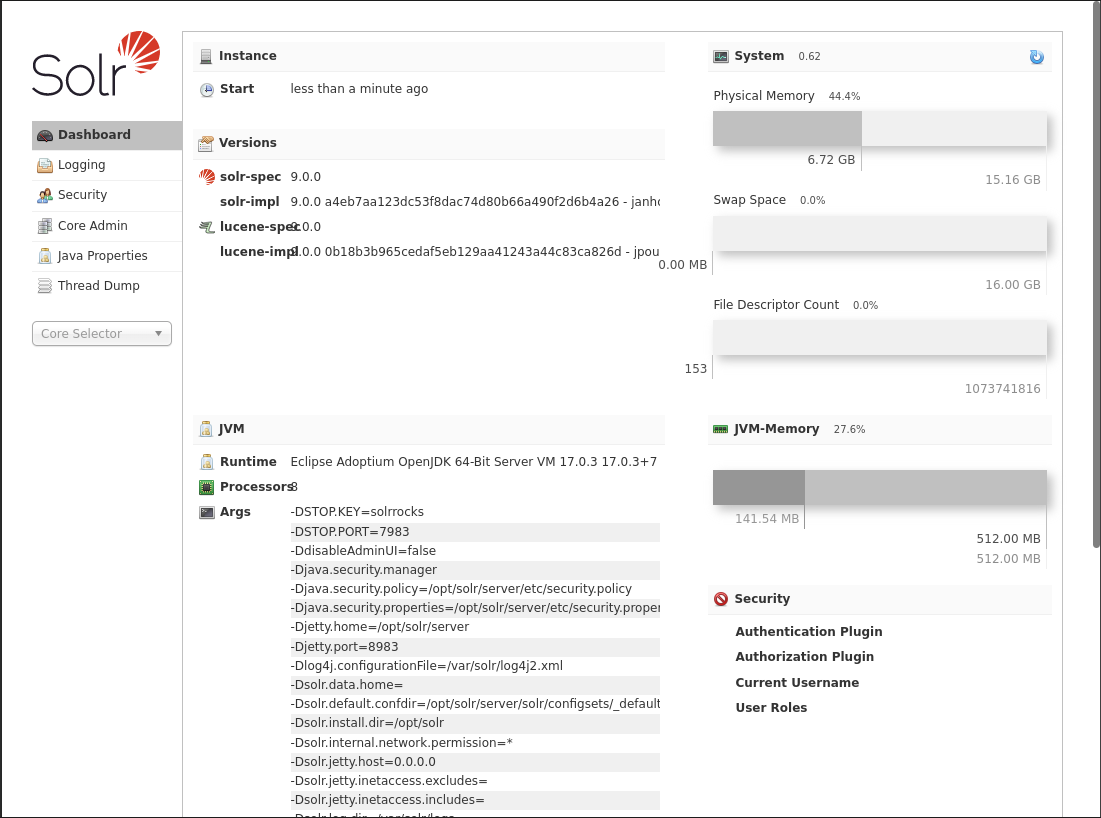
\includegraphics[width=0.75\linewidth]{files/images/solr-start-page}
	\caption{Solr start page}
	\label{fig:solr-start-page}
\end{figure}


In the ``Core Selector" drop-down, select the core we created (``songs\_jp") \\





From there, you can select ``Query" to start querying our dataset\dots (figure \ref{fig:solr-query}). \\

\newpage

\begin{figure}[h]
	\centering
	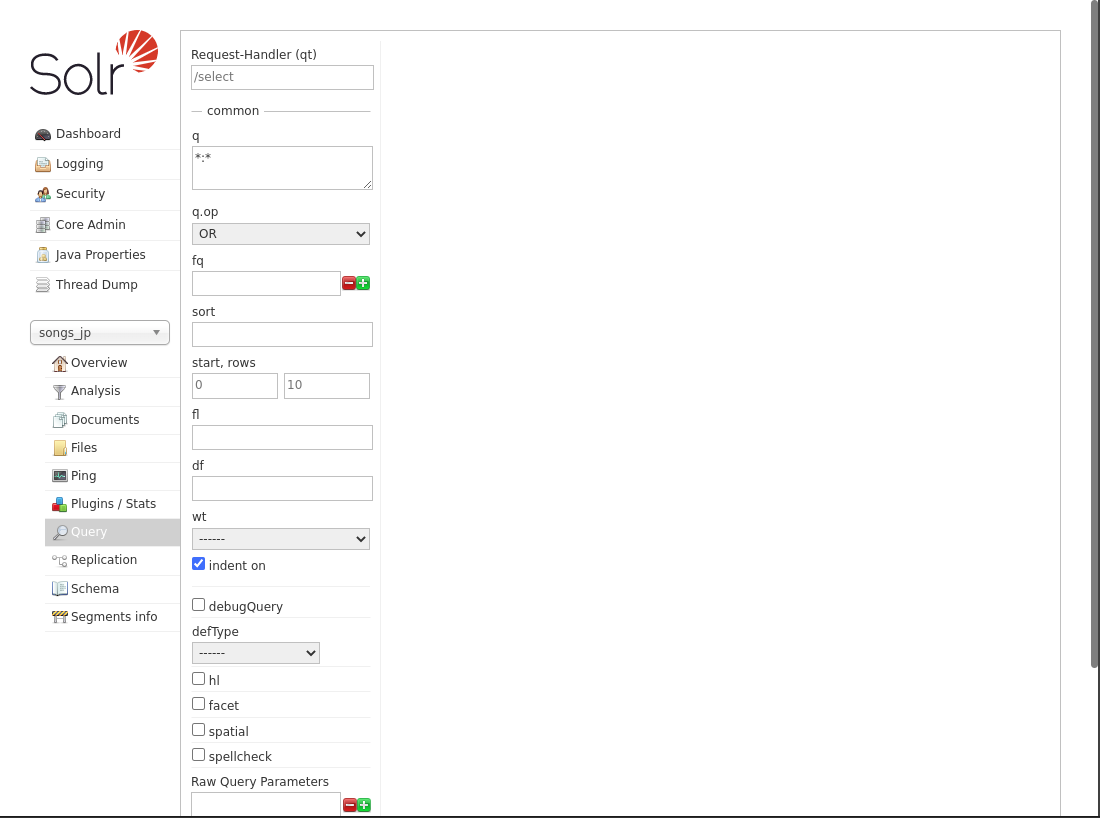
\includegraphics[width=0.75\linewidth]{files/images/solr-query}
	\caption{Solr query screen}
	\label{fig:solr-query}
\end{figure}

\bigskip

For our case study, we will mainly use the following fields from this screen:
\begin{itemize}
	\item \emph{fq}
	
	Stands for \emph{``filter query"}.
	
	We are going to use this field to filter out results (i.e. perform analysis only on a portion of our dataset).
	
	The default (\texttt{*:*}) does not filter anything.
	
	
	\item \emph{start, rows} \hfill default: \texttt{0,10}
	
	These are two positive integer values.
	
	They indicate which documents from the result-set to output: \texttt{start} (a.k.a. \emph{offset}), and number of \texttt{rows}.
	
	In our study, we are more interested in the result of the \faceting\ than the records themselves. 
	
	This means we will usually set both of these values to 0.
	
	\item \emph{facet}
	
	This is the field we are the most interested in.
	
	We will enable it most of the time.
	
	\begin{itemize}
		\item \emph{facet.field}
		
		This is the field on which to perform the \faceting.
		
		We will perform the \faceting\ on fields of either type \texttt{strings} (e.g. 
		
		\texttt{band\_str}), or indexed \texttt{text} (e.g. \texttt{lyrics\_txt\_ja})
		
		
		\item \emph{facet.mincount}  % \hfill default: \texttt{0}
			
		This field tells Solr to remove the \emph{facets} with a low document count. 
		
		For example, by setting \emph{facet.mincount} to \emph{1}, \emph{facets} with no documents will not appear.
		
		If this field is left empty, Solr will effectively use 0 as a default value.
		
		\item \emph{facet.limit}   \hfill default: \texttt{100}
		
		The maximum number of constraint counts (i.e. the number of facets for a field that are returned) that should be returned.
		
		A negative value means unlimited number of facets. 
		
		
	\end{itemize}
\end{itemize}


\bigskip
\bigskip

After filling up the fields, click on \emph{``Execute Query"} to display the results (figure~\ref{fig:solr-query-result}):

\begin{figure}[h]
	\centering
	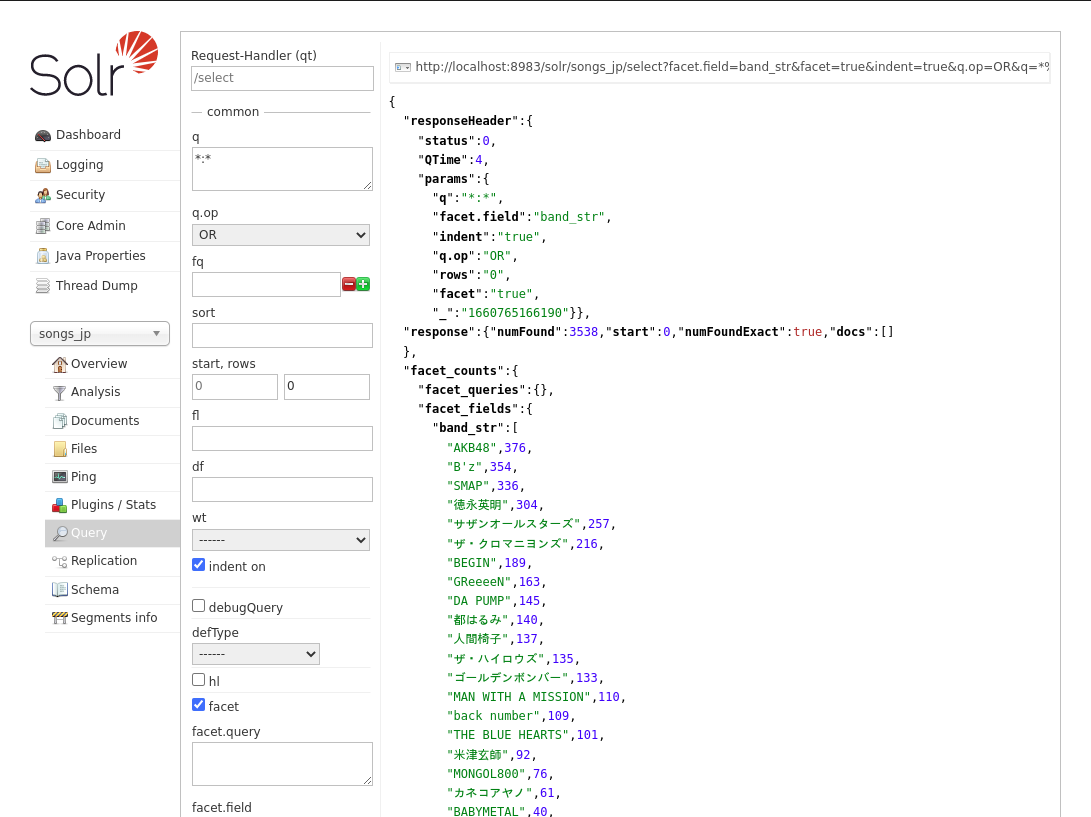
\includegraphics[width=0.75\linewidth]{files/images/solr-query-result}
	\caption{Solr query result}
	\label{fig:solr-query-result}
\end{figure}

\bigskip

Above the query result (in JSON), you can see a rather long URL. This shows the URL of web API for the current query (i.e. the kind of URL you will need to interact with Solr programmatically). \\

Clicking on the URL will display Solr's web API response, which is in JSON format (figure~\ref{fig:solr-web-api-result-json}):

\newpage

\begin{figure}[h]
	\centering
	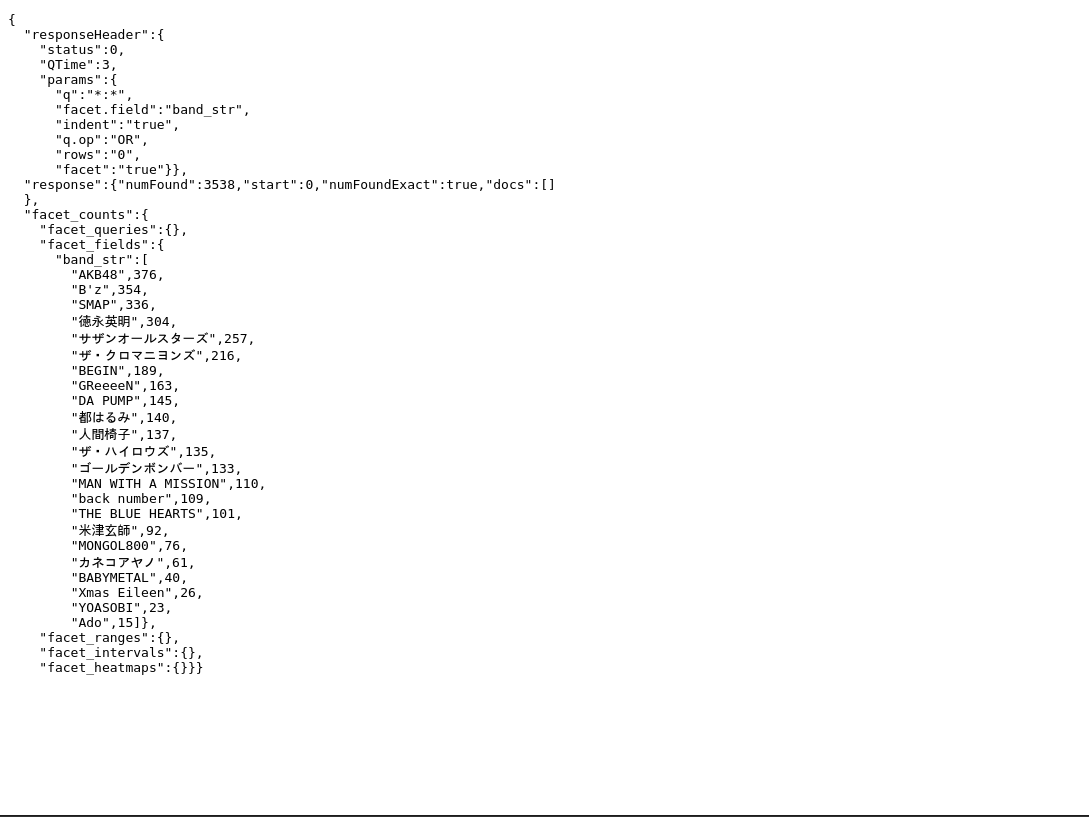
\includegraphics[width=0.75\linewidth]{files/images/solr-web-api-result}
	\caption{Solr - web API result}
	\label{fig:solr-web-api-result-json}
\end{figure}


\bigskip
\bigskip
\bigskip

Now that we are familiar with Solr, we all set to perform queries and analyse our dataset!




\newpage
% Copyright 2022 Pierre S. Caboche. All rights reserved.

\renewcommand{\currentPart}{Analysing lyrics}
\part{Analysing lyrics}   \label{analysing-lyrics}




\section{The dataset}

To create the dataset, I searched online for the lyrics from a variety of bands. \\

I tried to include popular bands, as well as a few personal favourites. I also tried to include bands from a variety of genres (Pop, Rock, Metal, Punk, \emph{Enka}\dots). \\

Having such a diversity would hopefully yield interesting results, as the bubbly vocabulary used by a Pop band might differ (at least in theory) from the sombre undertones of a metal band, or the melancholic verses of \emph{enka} songs. \\

Below are some of the bands I included for the study\dots \\


\subsection{Punk-Rock}

\subsubsection{THE BLUE HEARTS} \label{{THE BLUE HEARTS}}

THE BLUE HEARTS is one of my favourite bands, and what inspired me to write this paper (I was looking for the lyrics to some of their songs, and was interested in the writing style of the different band members). \\

\bigskip

THE BLUE HEARTS was a Japanese punk rock band active from 1985 to 1995. The band is very famous in Japan, and their songs have been featured in a lot of media (movies, series, video games, anime\dots) \\

THE BLUE HEARTS was mainly comprised of the following members:
\begin{itemize}
	\item Kōmoto Hiroto --- 甲本 ヒロト --- vocals, harmonica
	\item Mashima Masatoshi --- 真島 昌利 --- guitar, backing vocals
	\item Kawaguchi Junnosuke --- 河口 純之助 --- bass, backing vocals
	\item Kajiwara Tetsuya --- 梶原 徹也 --- drums
	\item Shirai Mikio --- 白井 幹夫 --- keyboards (support member)
\end{itemize}

\bigskip

The lyrics for THE BLUE HEARTS are credited to three of the band's members (Kōmoto, Mashima, and Kawaguchi). \\

Below is a selection of their songs, by author:

\begin{itemize}
	\item Kōmoto Hiroto --- 甲本 ヒロト
	\begin{itemize}
		\item \href{https://www.youtube.com/watch?v=RYC71PAuIKE}{リンダ リンダ} [Linda Linda]
		\item \href{https://www.youtube.com/watch?v=5yslQYshIAI}{ラブレター} [Love Letter]
		\item \href{https://www.youtube.com/watch?v=-p0Yqcx53O8}{情熱の薔薇} [Rose of Passion]
		\item \href{https://www.youtube.com/watch?v=t0rffmN7c6w}{歩く花} [The Walking Flower]
		\item \href{https://www.youtube.com/watch?v=BT-8_TFxohI}{キスしてほしい} [I want you to kiss me]
		\item \href{https://www.youtube.com/watch?v=xnQYtogdxyg}{夕暮れ} [Evening]
		\item 月の爆撃機 [Moon Bomber]
		\item 人にやさしく [Be kind to People]
		\item 1985
		\item 星をください [Give me a Star]
		\item M・O・N・K・E・Y
		\item 少年の詩 [Teenage Boy Poem]
		\item パーティー [PARTY]
	\end{itemize}
	
	\item Mashima Masatoshi --- 真島 昌利	
	\begin{itemize}
		\item \href{https://www.youtube.com/watch?v=BSkLe-EOq5U}{TRAIN-TRAIN}
		\item \href{https://www.youtube.com/watch?v=PQXMU1A8CjI}{青空} [Blue Sky]
		\item \href{https://www.youtube.com/watch?v=9yY5lwBT4mk}{TOO MUCH PAIN}
		\item \href{https://www.youtube.com/watch?v=egNok6oeMA0}{1000のバイオリン} [1000 violins]
		\item 夢 [Dream]
		\item 君のため [For you]
		\item 終わらない歌 [A never-ending Song]
		\item 僕はここに立っているよ [I'm standing here]	
	\end{itemize}
	
	\item Kawaguchi Junnosuke --- 河口 純之助	
	\begin{itemize}
		\item \href{https://www.youtube.com/watch?v=J4LKAFe82_w}{シンデレラ(灰の中から)} [Cinderella (from the ashes)]
		\item 心の救急車 [Ambulance of the Heart]
		\item 真夜中のテレフォン [Midnight Telephone]
	\end{itemize}
\end{itemize}

\bigskip


When the band broke up in 1995, Kōmoto Hiroto and Mashima Masatoshi went on to form a new band called ``The High-Lows", and then another band called ``The Cro-Magnons" after that (see~\ref{the-high-lows} and~\ref{the-cro-magnons}). \\


\bigskip

This will give us the opportunity to perform different types of queries:
\begin{itemize}
	\item most used words in songs by THE BLUE HEARTS (section~\ref{most-used-words-BLUE-HEARTS})
	
	\item most used words by the different songwriters throughout their career (not just as part of THE BLUE HEARTS), in section~\ref{most-used-words-by-songwriter}
\end{itemize}


\bigskip

After the band broke up, Kōmoto Hiroto and Mashima Masatoshi chose not to sing any of the songs from THE BLUE HEARTS, with a few occasional exceptions. \\

\bigskip

\subsubsection{The High-Lows (ザ・ハイロウズ)} \label{the-high-lows}

A Japanese punk rock band that was formed in 1995 by former members of THE BLUE HEARTS, Kōmoto Hiroto and Mashima Masatoshi (section~\ref{{THE BLUE HEARTS}}). \\

The band broke up in 2005. \\

Kōmoto and Mashima went on to form ``The Cro-Magnons".


\bigskip

\subsubsection{The Cro-Magnons (ザ・クロマニヨンズ)} \label{the-cro-magnons}

A Japanese punk rock band that was formed in 2006 by former members of THE BLUE HEARTS and ``The High-Lows", Kōmoto Hiroto and Mashima Masatoshi (section~\ref{{THE BLUE HEARTS}}). \\


\bigskip


\subsection{Pop}

\subsubsection{AKB48}

AKB48 (pronounced A.K.B. Forty-Eight) is an idol girl group named after the Akihabara (Akiba for short) area in Tokyo. \\

The band is immensely successful, and has sprouted multiple sister bands, both domestically (NMB48, HKT48, NGT48\dots) and abroad (JKT48, BNK48, MNL48, SNH48\dots) \\

The overall musical style of AKB48 is very girly, and sometimes flirtatious. \\

That being said, some of their songs really stand out:

\begin{itemize}
	\item \href{https://www.youtube.com/watch?v=fgESmgZ4ld8}{風は吹いている} [The Wind is Blowing] 
	\item \href{https://www.youtube.com/watch?v=JUbU6VLV6yI}{365日の紙飛行機} [365 Days Paper Plane]
	\item \href{https://www.youtube.com/watch?v=hUOc1yc8cH0}{桜の栞} [Cherry Blossom Bookmark]
	\item \href{https://www.youtube.com/watch?v=n24zp_wPC7E}{前しか向かねえ} [Only move forward]	
\end{itemize}





\bigskip
\subsection{Enka}

Enka (演歌) is a music genre typical from Japan. \\

Musically speaking, \emph{enka} resembles traditional Japanese music. In terms of lyrics, \emph{enka} songs include recurring themes such as: love, loss, loneliness, hardships, etc. to the point that it can be described as some sort of \emph{``Japanese blues"}. \\

\emph{Enka} songs are also often associated with a place and a season. \\

I've included songs from the following \emph{enka} singers in the dataset:

\subsubsection{Ishikawa Sayuri (石川さゆり)}

Born in 1958, Ishikawa Sayuri is a \emph{enka} singer who made her professional debut in 1973. She is one of the most-recognized and successful \emph{enka} singers in history. \\

Ishikawa's most popular songs include: 
\href{https://www.youtube.com/watch?v=OJxm9Lt-w6Y}{\furi{津軽/つがる,海峡/かいきょう, ・ /,冬/ふゆ,景色/けしき}} [Tsugaru Straight - Winter Scenery] (1977), and
\href{https://www.youtube.com/watch?v=yvc0LadtZUk}{\furi{天城/あまぎ,越/ご,え/}} [Walk Over the Amagi Pass] (1986).


\subsubsection{Miyako Harumi (都はるみ)}

Born in 1948, Miyako Harumi (née Kitamura Harumi) is a singer who made her debut in 1964 and is still active today, making television frequent appearances. \\

Although usually considered as an \emph{enka} singer, Miyako Harumi never thought of herself as such, arguing that the term \emph{``enka"} was not used in that context at the time of her début. \\

Popular song by Miyako Harumi include: \href{https://www.youtube.com/watch?v=QKmma_bRdQE}{\furi{北/きた,の/,宿/やど,から/}} [From an Inn in the North] (1975), and \href{https://www.youtube.com/watch?v=pltL1kuIU4}{\furi{大阪/おおさか,しぐれ/}} [Autumn Rain in Osaka] (1980). \\


\bigskip



\subsection{Metal}


\subsubsection{Ningen Isu (人間椅子)}

Ningen Isu (人間椅子 --- \emph{"The Human Chair"}) is a heavy metal band formed in 1987, and active ever since. The band is named after a short story by Edogawa Rampo, published in 1925. \\

The band is known for using some difficult and old words (from the Edo to Showa period, i.e. 1603 onwards), and the themes of their songs include: hell, the universe, Buddhism, etc. \\

For all these reasons, analysing the lyrics of their songs should be interesting (section \ref{most-used-words-Ningen-Isu}). \\

Personal favourites by Ningen Isu include:

\begin{itemize}
	\item \href{https://www.youtube.com/watch?v=CbI79e5iZKs}{\furi{無情/むじょう}のスキャット} [Heartless Scat]
	
	\item \href{https://www.youtube.com/watch?v=tKSjWKDSBmo}{杜子春} [Toshishun]
	
	\item \href{https://www.youtube.com/watch?v=CLoUY1kA4ZY}{なまはげ} [Namahage]
\end{itemize}

\bigskip

\subsubsection{BABYMETAL}

BABYMETAL (ベビーメタル) is a band often credited with the creation and success of a type of metal called ``kawaii metal" (\emph{cute metal}), a genre that combines heavy metal music and J-pop melodies. \\

The band formed in 2010. In October of 2021, the band released a cryptic video hinting a hiatus (or maybe the end of the band). \\

Some of their best songs include:

\begin{itemize}
	\item \href{https://www.youtube.com/watch?v=pDgqo6fcliY}{NO RAIN, NO RAINBOW}

	\item  \href{https://www.youtube.com/watch?v=nDqaTXqCN-Q}{イジメ、ダメ、ゼッタイ} [Bully, Never, Ever]
	
	\item \href{https://www.youtube.com/watch?v=WIKqgE4BwAY}{ギミチョコ!! --- Gimme chocolate!!} 
		
	\item \href{https://www.youtube.com/watch?v=oO7Y8NsnkRg}{PA PA YA!! (feat. F.HERO)}
	
	\item \href{https://www.youtube.com/watch?v=cK3NMZAUKGw}{メギツネ - MEGITSUNE}
	
	\item 紅月 --- アカツキ [Red moon]
\end{itemize}

\bigskip




\subsection{Other}

The dataset contains many more bands, and it would take too long to describe them all (the purpose of this section is to give you an idea of the type of band you will find in the dataset, and the reasons why some of the bands were added). \\

The list of bands in the dataset (and the number of songs for each band) can be found on page~\pageref*{query-list-of-bands} in section~\emph{\longref{query-list-of-bands}} \\






\newpage
\section{Exploring the dataset} \label{exploring-dataset}

\subsection{Queries and results}

Solr returns results in JSON format. \\

In this article, we show only \emph{part} of the results returned by Solr, in a more readable form (e.g. in textual form, as a table). \\

We also add some extra information (such as pronunciations, and common English translations) for convenience to the reader. \\

\bigskip

Below are the descriptions of the column names:

\begin{longtable}{l p{11.5cm}}


\emph{"numFound"} :& The total number of documents (i.e. songs) in the result-set. \\
& \\
	
\emph{Band} :& The band (バンド), or artist name.\\
& \\
&
This is the key returned when performing some \faceting\ on field: \texttt{band\_str}.
\\

& \\


\emph{Songwriter} :& The songwriter. (\furi{作詞家/さくしか})\\
& \\
&
This is the key returned when performing some \faceting\ on field: \texttt{lyrics\_by\_str}. 
(section \ref{songwriters-TBH}) 
\\



& \\


\emph{Lexeme}: &
Lexeme (\furi{語彙素/ごいそ})
\\


& 
A Japanese word, as it would appear in its dictionary form (i.e. without \emph{inflection})
\\
& \\

\emph{何曲}: &  \furi{何/なん,曲/きょく} -- number of songs\\


& \emph{nankyoku} -- \emph{``How many songs?", ``What songs?"} \\

& \\
&
This column represents the number of songs for each item in the result-set.  \newline
This is the value returned by Solr when performing some \faceting\ (on the fields like: \texttt{band\_str}, \texttt{lyrics\_by\_str}, \texttt{lyrics\_txt\_ja}), as we will see in the rest of this section. \\

%(何曲 -- \emph{nankyoku} -- \emph{``How many songs?", ``What songs?"})

& \\

\emph{Pronunc.}: 
&
\emph{(not part of the result-set returned by Solr; this column is been added for the convenience to the reader)}
\\
& \\
& Shows the most common pronunciations for a particular \emph{lexeme} (some words may have more than one pronunciation), in \emph{romaji}. \\

& \\

\emph{Meanings}:
&
\emph{(not part of the result-set returned by Solr; this column is been added for the convenience to the reader)}
\\
& \\
& Shows the most common meanings or English translations for a particular \emph{lexeme}
\\


\end{longtable}

\newpage

\subsection{General queries}  \label{general-queries}




\subsubsection{List of bands (whole dataset)} \label{query-list-of-bands}

Question: \\
\emph{``Which bands (or solo artists) are in the dataset? (and how many songs do they have?)"} \\


Query:

\begin{tabular}{|l|l|}
	\hline
	& \\
	rows: & 0 \\
	facet: & true \\
	facet.field: & band\_str \\
	& \\
	\hline
\end{tabular}



\bigskip
Result: \\

"numFound":
7263


\begin{longtable}{|l l|r|}
	\hline
	\multicolumn{2}{|c|}{Band (バンド)} & 
	\multicolumn{1}{|c|}{何曲}
	\\
	\hline
	& & \\
	\endhead
	
	\hline
	\endfoot
	
	松任谷由実 & \emph{Matsutōya Yumi} & 417 \\
AKB48 & & 376 \\
B'z & & 354 \\
SMAP & & 336 \\
徳永英明 & \emph{Tokunaga Hideaki} & 304 \\
ゆず & \emph{Yuzu} & 292 \\
JAM Project & & 264 \\
サザンオールスターズ & \emph{Southern All Stars} & 257 \\
aiko & & 256 \\
石川さゆり & \emph{Ishikawa Sayuri} & 249 \\
Mr.Children & & 244 \\
DREAMS COME TRUE & & 243 \\
ザ・クロマニヨンズ & \emph{The Cro-Magnons} & 216 \\
ORANGE RANGE & & 190 \\
BEGIN & & 189 \\
RADWIMPS & & 177 \\
GReeeeN & & 163 \\
いきものがかり & \emph{Ikimonogakari} & 152 \\
LiSA & & 150 \\
L'Arc~en~Ciel & & 149 \\
DA PUMP & & 145 \\
都はるみ & \emph{Miyako Harumi} & 140 \\
人間椅子 & \emph{Ningen Isu} & 137 \\
ザ・ハイロウズ & \emph{The High-Lows} & 135 \\
ゴールデンボンバー & \emph{Golden Bomber} & 133 \\
BUMP OF CHICKEN & & 132 \\
Aimer & & 131 \\
fripSide & & 131 \\
Superfly & & 130 \\
ONE OK ROCK & & 129 \\
GACKT & & 125 \\
MAN WITH A MISSION & & 110 \\
back number & & 109 \\
Kiroro & & 102 \\
THE BLUE HEARTS & & 101 \\
米津玄師 & \emph{Younezu Kenshi} & 92 \\
MONGOL800 & & 76 \\
河島英五 & \emph{Kawashima Eigo} & 62 \\
カネコアヤノ & \emph{Kaneko Ayano} & 61 \\
BABYMETAL & & 40 \\
Xmas Eileen & & 26 \\
YOASOBI & & 23 \\
Ado & & 15 \\

	& & \\
\end{longtable}

\bigskip



\subsubsection{Most used words (whole dataset)} \label{most-used-words-dataset}

Question: \\
\emph{``Which words appear the most in our dataset?"} \\

Query:

\begin{tabular}{| l | l |}
	\hline
	& \\
	start, rows: & 0, 0 \\
	facet: & true \\
	facet.field: & lyrics\_txt\_ja \\
	%	facet.mincount: & 1 \\
	& \\
	\hline
\end{tabular}




\bigskip
Result: \\




\begin{myLongTable}{Most used words in songs stored in our dataset}
	人 & \emph{hito} & person & 2800 \\
今 & \emph{ima} & now & 2729 \\
君 & \emph{kimi} & you, buddy, pal & 2574 \\
何 & \emph{nani} &  what & 2540 \\
心 & \emph{kokoro} & heart, mind, spirit& 2296 \\
誰 & \emph{dare} & who & 2238 \\
僕 & \emph{boku} &  I, me (Pronoun, Male term) & 2185 \\
夢 & \emph{yume} & dream & 2150 \\
そう & \emph{sou} & looking like & 2143 \\
中 & \emph{naka} & inside & 1998 \\
日 & \emph{hi, nichi} & day & 1949 \\
いい & \emph{ii} & good, excellent, fine, nice & 1915 \\
もう & \emph{mou} & already, yet, by now& 1890 \\
時 & \emph{toki} & time, hour, moment & 1874 \\
見る & \emph{miru} & to see & 1873 \\
あなた & \emph{anata} & you & 1850 \\
あの & \emph{ano} & that, those, the & 1747 \\
手 & \emph{te} & hand, arm & 1706 \\
空 & \emph{sora} & sky & 1615 \\
行く & \emph{iku} & to go & 1571 \\
胸 & \emph{mune} & chest, breast, heart & 1569 \\
知る & \emph{shiru} &  to be aware of, to know, to be conscious of & 1497 \\
風 & \emph{kaze} & wind & 1490 \\
愛 & \emph{ai} & love & 1473 \\
涙 & \emph{namida} & tears & 1457 \\
まま & \emph{mama} & as it is, as one likes & 1434 \\
目 & \emph{me} & eye & 1426 \\
くれる & \emph{kureru} & to give, to let (one) have & 1415 \\
夜 & \emph{yoru} & evening, night & 1407 \\
忘れる & \emph{wasureru} & to forget & 1397 \\
明日 & \emph{ashita, asu} & tomorrow, (only "asu") the near future & 1395 \\
生きる & \emph{ikiru} & to live, to exist & 1389 \\
一 & \emph{ichi} & one & 1384 \\
どこ & \emph{doko} & where, what place & 1366 \\
言う & \emph{iu} & to say & 1364 \\
笑う & \emph{warau} & to laugh & 1350 \\
く & \emph{ku} & ward, borough, city (in Tokyo) & 1346 \\
声 & \emph{koe} & voice & 1335 \\
言葉 & \emph{kotoba} & word, phrase& 1325 \\
今日 & \emph{kyou} & today & 1324 \\
ゆく & \emph{iku} & 行く:  to go & 1282 \\
くる & \emph{kuru} & 来:  to come & 1270 \\
世界 & \emph{sekai} & the world, society, the universe & 1257 \\
いつ & \emph{itsu} & when, at what time & 1253 \\
いつも & \emph{itsumo} & always, all the time, at all times & 1245 \\
来る & \emph{kuru} & to come & 1232 \\
いく & \emph{iku} & 行く:  to go & 1226 \\
きっと & \emph{kitto} & surely, undoubtedly, almost certainly & 1216 \\
泣く & \emph{naku} & to cry, to weep, to sob & 1176 \\
見える & \emph{mieru} & to be seen, to be in sight, to appear & 1164 \\
you & \emph{-} & - & 1152 \\
自分 & \emph{jibun} & I, me, myself, yourself, oneself (Pronoun) & 1136 \\
私 & \emph{watashi} & I, me (Pronoun, slightly formal or feminine) & 1130 \\
i & \emph{-} & - & 1113 \\
前 & \emph{mae} & in front (of), before & 1097 \\
消える & \emph{kieru} & to go out, to vanish, to disappear & 1096 \\
しまう & \emph{shimau} & to finish, to stop, to put an end to & 1080 \\
いつか & \emph{itsuka} & sometime, someday, one day & 1078 \\
歩く & \emph{aruku} & to walk & 1065 \\
そんな & \emph{sonna} & such, that sort of, that kind of & 1064 \\
恋 & \emph{koi} & (romantic) love & 1060 \\
変わる & \emph{kawaru} & to change, to be transformed, to be altered & 1055 \\
ずっと & \emph{zutto} & continuously, throughout & 1040 \\
事 & \emph{koto} & thing, matter & 1039 \\
未来 & \emph{mirai} & the future (usually distant) & 1009 \\
まだ & \emph{mada} & still, as yet, only & 997 \\
信じる & \emph{shinjiru} & to believe, to place trust in, to have faith in & 994 \\
思う & \emph{omou} & to think, to consider, to believe, to reckon& 972 \\
街 & \emph{gai} & \dots\ street, \dots\ quarter, \dots\ district & 969 \\
気 & \emph{ki} & spirit, mind, heart & 954 \\
二 & \emph{ni} & two & 944 \\
待つ & \emph{matsu} & to wait & 932 \\
みる & \emph{miru} & 見る:  to see & 913 \\
少し & \emph{sukoshi} & a little, a few & 910 \\
好き & \emph{suki} & liked, well-liked, in love (with) & 891 \\
光 & \emph{hikari} & light & 886 \\
道 & \emph{machi} & road, path, street, lane & 886 \\
日々 & \emph{hibi} & the everyday & 861 \\
強い & \emph{tsuyoi} & strong, potent, competent, tough, powerful & 860 \\
僕ら & \emph{bokura} & we (Pronoun, Male term) & 849 \\
想い & \emph{omoi} & thought & 844 \\
the & \emph{-} & - & 836 \\
遠い & \emph{toi} & far, distant, far away & 820 \\
度 & \emph{do} & (counter for occurrences) & 818 \\
わかる & \emph{wakaru} & 分かる:  to understand, to comprehend, to grasp & 804 \\
優しい & \emph{yasashii} & tender, kind, gentle, affectionate & 788 \\
気持ち & \emph{kimochi} & feeling, sensation, mood, state of mind & 786 \\
笑顔 & \emph{egaho} & smiling face, smile & 784 \\
終わる & \emph{owaru} & to end, to come to an end, to close, to finish & 766 \\
続ける & \emph{tsuzukeru} & to continue, to keep up, to keep on & 760 \\
時間 & \emph{jikan} & time & 759 \\
my & \emph{-} & - & 749 \\
顔 & \emph{kao} & face, visage & 735 \\
雨 & \emph{ame} & rain& 728 \\
同じ & \emph{onaji} & same, identical, equal, similar, alike & 725 \\
to & \emph{-} & - & 723 \\
探す & \emph{sagasu} & to search for, to look for, to hunt for, to seek & 711 \\
星 & \emph{hoshi} & star & 710 \\
出る & \emph{deru} & 出る:  to leave, to exit, to go out & 700 \\

	& & & \\
\end{myLongTable}

\bigskip
\bigskip





\subsubsection{List of songwriters (band: ``THE BLUE HEARTS")}  \label{songwriters-TBH}

Question: \\
\emph{``How many different songwriters are there in the band ``THE BLUE HEARTS"? "} \\


Query:

\begin{tabular}{| l |  l |}
	\hline
	& \\
	fq: & band\_str:"THE BLUE HEARTS" \\
	start, rows: & 0, 0 \\
	facet: & true \\
	facet.field: & lyrics\_by\_str \\
	facet.mincount: & 1 \\
	& \\
	\hline
\end{tabular}


\bigskip
Result: \\

"numFound":101

\begin{longtable}{|l l|l|}
	\hline
	\multicolumn{2}{|c|}{Songwriter (作詞家)} & 
	\multicolumn{1}{|c|}{何曲}
	\\
	\hline
	& & \\
	\endhead
	
	\hline
	\endfoot
	
	真島昌利 & Mashima Masatoshi & 50 \\
	甲本ヒロト & Kōmoto Hiroto & 45 \\
	河口純之助 & Kawaguchi Junnosuke & 5 \\
	甲本ヒロト・真島昌利 & Kōmoto Hiroto ・ & 1 \\
	& Mashima Masatoshi& \\
	& & \\
\end{longtable}

\bigskip






\newpage

\subsection{Most used words, by band} \label{most-used-words-by-band}

In this section, we are going to find the most used for the following artists:

\begin{itemize}
	\item THE BLUE HEARTS
	\item AKB48
	\item SMAP
	\item Ningen isu
	\item Kaneko Ayano
\end{itemize}

\bigskip


\subsubsection{Most used words (band: ``THE BLUE HEARTS")} \label{most-used-words-BLUE-HEARTS}

Question: \\
\emph{``Which words appear most often in songs by the band ``THE BLUE HEARTS"? "} \\

Query:

\begin{tabular}{| l |  l |}
	\hline
	& \\
	fq: & band\_str:"THE BLUE HEARTS" \\
	start, rows: & 0, 0 \\
	facet: & true \\
	facet.field: & lyrics\_txt\_ja \\
	%	facet.mincount: & 1 \\
	& \\
	\hline
\end{tabular}


\bigskip
Result: \\

"numFound":101

\begin{myLongTable}{Most used words in songs by the band ``THE BLUE HEARTS"}
	僕 & \emph{boku} &  I, me (Pronoun, Male term) & 42 \\
誰 & \emph{dare} & who & 36 \\
何 & \emph{nani} &  what & 33 \\
事 & \emph{koto} & thing, matter & 29 \\
人 & \emph{hito} & person & 29 \\
行く & \emph{iku} & to go & 25 \\
夜 & \emph{yoru} & evening, night & 24 \\
見る & \emph{miru} & to see & 24 \\
風 & \emph{kaze} & wind & 24 \\
今 & \emph{ima} & now & 22 \\
いい & \emph{ii} & good, excellent, fine, nice & 21 \\
中 & \emph{naka} & inside & 21 \\
やる & \emph{yaru} & to do, to undertake, to perform & 19 \\
笑う & \emph{warau} & to laugh & 19 \\
いく & \emph{iku} & 行く:  to go & 17 \\
どこ & \emph{doko} & where, what place & 17 \\
君 & \emph{kimi} & you, buddy, pal & 17 \\
時 & \emph{toki} & time, hour, moment & 17 \\
死ぬ & \emph{shinu} & to die & 17 \\
くる & \emph{kuru} & 来:  to come & 16 \\
そう & \emph{sou} & looking like & 16 \\
今日 & \emph{kyou} & today & 16 \\
いつ & \emph{itsu} & when, at what time & 15 \\
夢 & \emph{yume} & dream & 15 \\
一 & \emph{ichi} & one & 14 \\
言う & \emph{iu} & to say & 14 \\
そんな & \emph{sonna} & such, that sort of, that kind of & 13 \\
声 & \emph{koe} & voice & 13 \\
手 & \emph{te} & hand, arm & 13 \\
星 & \emph{hoshi} & star & 13 \\
空 & \emph{sora} & sky & 13 \\
雨 & \emph{ame} & rain& 13 \\
もう & \emph{mou} & already, yet, by now& 12 \\
心 & \emph{kokoro} & heart, mind, spirit& 12 \\
聞く & \emph{kiku} & to hear& 12 \\
言葉 & \emph{kotoba} & word, phrase& 12 \\
あげる & \emph{ageru} & 上げる:  to raise, to elevate & 11 \\
あなた & \emph{anata} & you & 11 \\
しまう & \emph{shimau} & to finish, to stop, to put an end to & 11 \\
上 & \emph{ue} & above, up, over & 11 \\
世界 & \emph{sekai} & the world, society, the universe & 11 \\
前 & \emph{mae} & in front (of), before & 11 \\
忘れる & \emph{wasureru} & to forget & 11 \\
明日 & \emph{ashita, asu} & tomorrow, (only "asu") the near future & 11 \\
気 & \emph{ki} & spirit, mind, heart & 11 \\
涙 & \emph{namida} & tears & 11 \\
生きる & \emph{ikiru} & to live, to exist & 11 \\
街 & \emph{gai} & \dots\ street, \dots\ quarter, \dots\ district & 11 \\
見える & \emph{mieru} & to be seen, to be in sight, to appear & 11 \\
遠い & \emph{toi} & far, distant, far away & 11 \\
みんな & \emph{minna} & everyone, everybody, all & 10 \\
俺 & \emph{ore} & I, me (Pronoun, Male term, rough or arrogant) & 10 \\
吹く & \emph{fuku} & to blow (of the wind) & 10 \\
日 & \emph{hi, nichi} & day & 10 \\
気持ち & \emph{kimochi} & feeling, sensation, mood, state of mind & 10 \\
泣く & \emph{naku} & to cry, to weep, to sob & 10 \\
目 & \emph{me} & eye & 10 \\
あの & \emph{ano} & that, those, the & 9 \\
つける & \emph{tsukeru} &  & 9 \\
どう & \emph{dou} & how, in what way, how about & 9 \\
まま & \emph{mama} & as it is, as one likes & 9 \\
みたい & \emph{mitai} & -like, sort of, similar to, resembling & 9 \\
本当 & \emph{hontou} & truth, reality, actuality, fact & 9 \\
生まれる & \emph{umareru} & to be born & 9 \\
道 & \emph{machi} & road, path, street, lane & 9 \\
く & \emph{ku} & ward, borough, city (in Tokyo) & 8 \\
くれる & \emph{kureru} & to give, to let (one) have & 8 \\
すぎる & \emph{sugiru} & to pass through, to pass by & 8 \\
つく & \emph{tsuku} & 着く:  to arrive at, to reach & 8 \\
でる & \emph{deru} & 出る:  to leave, to exit, to go out & 8 \\
なれる & \emph{nareru} & 慣れる:  to get used to & 8 \\
ゆく & \emph{iku} & 行く:  to go & 8 \\
夏 & \emph{natsu} & summer & 8 \\
悪い & \emph{warui} & bad, poor, undesirable & 8 \\
来る & \emph{kuru} & to come & 8 \\
欲しい & \emph{hoshii} & wanted, wished for, in need of, desired & 8 \\
歌う & \emph{utau} & to sing & 8 \\
者 & \emph{mono, sha} & person & 8 \\
達 & \emph{tachi} & (pluralizing suffix) & 8 \\
降る & \emph{furu} & to fall (of rain, snow, ash, etc.), to come down & 8 \\
飛ばす & \emph{tobasu} & to let fly, to make fly, to skip over, to leave out & 8 \\
ああ & \emph{aa} & ah!, oh!, alas! & 7 \\
いける & \emph{ikeru} &  & 7 \\
かける & \emph{kakeru} & & 7 \\
ずっと & \emph{zutto} & continuously, throughout & 7 \\
たくさん & \emph{takusan} & a lot, lots, plenty, many, a large number, much & 7 \\
みる & \emph{miru} & 見る:  to see & 7 \\
下 & \emph{shita} & below, down, under, & 7 \\
世の中 & \emph{yononaka} & society, the world, the times & 7 \\
今夜 & \emph{konya} & this evening, tonight & 7 \\
奴 & \emph{yatsu} & fellow, guy, chap (Derogatory) & 7 \\
少し & \emph{sukoshi} & a little, a few & 7 \\
思い出 & \emph{omoide} & memories, recollections, reminiscence & 7 \\
方 & \emph{hou} & direction, way, side & 7 \\
月 & \emph{tsuki} & moon & 7 \\
楽しい & \emph{tanoshii} & enjoyable, fun, pleasant & 7 \\
歴史 & \emph{rekishi} & history & 7 \\
続く & \emph{tsuzuku} & to continue, to last, to go on & 7 \\
言える & \emph{ieru} & to be possible to say, to be able to say & 7 \\

	& & & \\
\end{myLongTable}


\bigskip
\bigskip




\subsubsection{Most used words (band: ``AKB48")}

Question: \\
\emph{``Which words appear most often in songs by the band ``AKB48"? "} \\


\begin{tabular}{| l |  l |}
	\hline
	& \\
	fq: & band\_str:"AKB48" \\
	start, rows: & 0, 0 \\
	facet: & true \\
	facet.field: & lyrics\_by\_str \\
	%	facet.mincount: & 1 \\
	& \\
	\hline
\end{tabular}



\bigskip
Result: \\

"numFound":376

\begin{myLongTable}{Most used words in songs by the band ``AKB48"}
	人 & \emph{hito} & person & 216 \\
誰 & \emph{dare} & who & 204 \\
何 & \emph{nani} &  what & 191 \\
私 & \emph{watashi} & I, me (Pronoun, slightly formal or feminine) & 177 \\
今 & \emph{ima} & now & 167 \\
夢 & \emph{yume} & dream & 160 \\
愛 & \emph{ai} & love & 146 \\
どこ & \emph{doko} & where, what place & 145 \\
来る & \emph{kuru} & to come & 140 \\
心 & \emph{kokoro} & heart, mind, spirit& 137 \\
そう & \emph{sou} & looking like & 136 \\
いい & \emph{ii} & good, excellent, fine, nice & 133 \\
一 & \emph{ichi} & one & 128 \\
見る & \emph{miru} & to see & 128 \\
中 & \emph{naka} & inside & 124 \\
日 & \emph{hi, nichi} & day & 123 \\
自分 & \emph{jibun} & I, me, myself, yourself, oneself (Pronoun) & 122 \\
行く & \emph{iku} & to go & 119 \\
恋 & \emph{koi} & (romantic) love & 117 \\
あなた & \emph{anata} & you & 116 \\
風 & \emph{kaze} & wind & 111 \\
君 & \emph{kimi} & you, buddy, pal & 109 \\
空 & \emph{sora} & sky & 108 \\
時 & \emph{toki} & time, hour, moment & 107 \\
僕 & \emph{boku} &  I, me (Pronoun, Male term) & 103 \\
ずっと & \emph{zutto} & continuously, throughout & 100 \\
未来 & \emph{mirai} & the future (usually distant) & 97 \\
目 & \emph{me} & eye & 96 \\
言う & \emph{iu} & to say & 95 \\
涙 & \emph{namida} & tears & 93 \\
あの & \emph{ano} & that, those, the & 90 \\
忘れる & \emph{wasureru} & to forget & 90 \\
気づく & \emph{kizuku} & to notice, to recognise, to become aware of & 90 \\
道 & \emph{machi} & road, path, street, lane & 90 \\
いつ & \emph{itsu} & when, at what time & 89 \\
前 & \emph{mae} & in front (of), before & 88 \\
好き & \emph{suki} & liked, well-liked, in love (with) & 88 \\
生きる & \emph{ikiru} & to live, to exist & 88 \\
手 & \emph{te} & hand, arm & 87 \\
くれる & \emph{kureru} & to give, to let (one) have & 86 \\
わかる & \emph{wakaru} & 分かる:  to understand, to comprehend, to grasp & 85 \\
今日 & \emph{kyou} & today & 85 \\
信じる & \emph{shinjiru} & to believe, to place trust in, to have faith in & 85 \\
知る & \emph{shiru} &  to be aware of, to know, to be conscious of & 85 \\
胸 & \emph{mune} & chest, breast, heart & 84 \\
まま & \emph{mama} & as it is, as one likes & 82 \\
しまう & \emph{shimau} & to finish, to stop, to put an end to & 80 \\
歩く & \emph{aruku} & to walk & 78 \\
いつも & \emph{itsumo} & always, all the time, at all times & 76 \\
きっと & \emph{kitto} & surely, undoubtedly, almost certainly & 76 \\
いつか & \emph{itsuka} & sometime, someday, one day & 73 \\
思う & \emph{omou} & to think, to consider, to believe, to reckon& 73 \\
見える & \emph{mieru} & to be seen, to be in sight, to appear & 73 \\
すべて & \emph{subete} & 全て:  everything, all, the whole & 72 \\
世界 & \emph{sekai} & the world, society, the universe & 71 \\
声 & \emph{koe} & voice & 69 \\
待つ & \emph{matsu} & to wait & 68 \\
2 & & & 66 \\
度 & \emph{do} & (counter for occurrences) & 66 \\
夜 & \emph{yoru} & evening, night & 65 \\
どんな & \emph{donna} & what kind of, what sort of & 64 \\
みたい & \emph{mitai} & -like, sort of, similar to, resembling & 64 \\
みんな & \emph{minna} & everyone, everybody, all & 63 \\
愛しい & \emph{itoshii} & lovely, dear, beloved, darling, dearest & 63 \\
なれる & \emph{nareru} & 慣れる:  to get used to & 62 \\
欲しい & \emph{hoshii} & wanted, wished for, in need of, desired & 61 \\
そんな & \emph{sonna} & such, that sort of, that kind of & 60 \\
もう & \emph{mou} & already, yet, by now& 60 \\
大人 & \emph{otona} & adult, grown-up & 60 \\
みる & \emph{miru} & 見る:  to see & 58 \\
合う & \emph{au} & to come together, to merge, to unite, to meet & 58 \\
場所 & \emph{basho} & place, location, spot, position & 58 \\
思い出 & \emph{omoide} & memories, recollections, reminiscence & 58 \\
明日 & \emph{ashita, asu} & tomorrow, (only "asu") the near future & 58 \\
すぎる & \emph{sugiru} & to pass through, to pass by & 57 \\
変わる & \emph{kawaru} & to change, to be transformed, to be altered & 57 \\
気持ち & \emph{kimochi} & feeling, sensation, mood, state of mind & 57 \\
なぜ & \emph{naze} & why, how & 55 \\
先 & \emph{saki} & head (of a line), front & 53 \\
友達 & \emph{tomodachi} & friend, companion & 53 \\
気 & \emph{ki} & spirit, mind, heart & 53 \\
言葉 & \emph{kotoba} & word, phrase& 53 \\
ひとつ & \emph{hitotsu} & one (counter) & 52 \\
出す & \emph{dasu} & to take out, to get out & 52 \\
時間 & \emph{jikan} & time & 52 \\
やさしい & \emph{yasashii} & 優しい:  tender, kind, gentle, affectionate & 51 \\
あきらめる & \emph{akirameru} & 諦める:  to give up & 49 \\
く & \emph{ku} & ward, borough, city (in Tokyo) & 49 \\
しあわせ & \emph{shiawase} & 幸せ:  happiness, good fortune, luck, blessing & 49 \\
街 & \emph{gai} & \dots\ street, \dots\ quarter, \dots\ district & 49 \\
もっと & \emph{motto} & (some) more, even more, longer, further & 48 \\
やる & \emph{yaru} & to do, to undertake, to perform & 48 \\
長い & \emph{nagai} & long (distance, length), long (time), prolonged & 47 \\
すぐ & \emph{sugu} & immediately, at once, right away, directly & 46 \\
キス & \emph{kissu} & kiss & 46 \\
探す & \emph{sagasu} & to search for, to look for, to hunt for, to seek & 46 \\
どう & \emph{dou} & how, in what way, how about & 45 \\
太陽 & \emph{taiyou} & sun & 45 \\
教える & \emph{oshieru} & to teach, to instruct & 45 \\

	& & & \\
\end{myLongTable}







\bigskip
\subsubsection{Most used words (band: ``SMAP")}

Question: \\
\emph{``Which words appear most often in songs by the band ``SMAP"? "} \\


\begin{tabular}{| l |  l |}
	\hline
	& \\
	fq: & band\_str:"SMAP" \\
	start, rows: & 0, 0 \\
	facet: & true \\
	facet.field: & lyrics\_by\_str \\
	%	facet.mincount: & 1 \\
	& \\
	\hline
\end{tabular}

\bigskip
Result: \\

"numFound":336

\begin{myLongTable}{Most used words in songs by ``Kaneko Ayano"}
	君 & \emph{kimi} & you, buddy, pal & 201 \\
僕 & \emph{boku} &  I, me (Pronoun, Male term) & 159 \\
人 & \emph{hito} & person & 147 \\
そう & \emph{sou} & looking like & 139 \\
誰 & \emph{dare} & who & 114 \\
何 & \emph{nani} &  what & 113 \\
今 & \emph{ima} & now & 111 \\
いい & \emph{ii} & good, excellent, fine, nice & 107 \\
時 & \emph{toki} & time, hour, moment & 98 \\
中 & \emph{naka} & inside & 95 \\
夢 & \emph{yume} & dream & 95 \\
心 & \emph{kokoro} & heart, mind, spirit& 95 \\
見る & \emph{miru} & to see & 94 \\
日 & \emph{hi, nichi} & day & 93 \\
胸 & \emph{mune} & chest, breast, heart & 89 \\
いつも & \emph{itsumo} & always, all the time, at all times & 81 \\
きっと & \emph{kitto} & surely, undoubtedly, almost certainly & 80 \\
もう & \emph{mou} & already, yet, by now& 79 \\
気持ち & \emph{kimochi} & feeling, sensation, mood, state of mind & 79 \\
空 & \emph{sora} & sky & 78 \\
夜 & \emph{yoru} & evening, night & 77 \\
言う & \emph{iu} & to say & 77 \\
you & \emph{-} & - & 75 \\
く & \emph{ku} & ward, borough, city (in Tokyo) & 75 \\
いつ & \emph{itsu} & when, at what time & 74 \\
行く & \emph{iku} & to go & 73 \\
手 & \emph{te} & hand, arm & 72 \\
生きる & \emph{ikiru} & to live, to exist & 72 \\
あの & \emph{ano} & that, those, the & 71 \\
明日 & \emph{ashita, asu} & tomorrow, (only "asu") the near future & 71 \\
愛 & \emph{ai} & love & 70 \\
まま & \emph{mama} & as it is, as one likes & 69 \\
一 & \emph{ichi} & one & 68 \\
恋 & \emph{koi} & (romantic) love & 68 \\
そんな & \emph{sonna} & such, that sort of, that kind of & 67 \\
今日 & \emph{kyou} & today & 67 \\
笑う & \emph{warau} & to laugh & 67 \\
くる & \emph{kuru} & 来:  to come & 66 \\
二 & \emph{ni} & two & 66 \\
風 & \emph{kaze} & wind & 66 \\
どこ & \emph{doko} & where, what place & 63 \\
忘れる & \emph{wasureru} & to forget & 63 \\
ずっと & \emph{zutto} & continuously, throughout & 62 \\
僕ら & \emph{bokura} & we (Pronoun, Male term) & 61 \\
街 & \emph{gai} & \dots\ street, \dots\ quarter, \dots\ district & 61 \\
涙 & \emph{namida} & tears & 59 \\
目 & \emph{me} & eye & 59 \\
知る & \emph{shiru} &  to be aware of, to know, to be conscious of & 59 \\
ゆく & \emph{iku} & 行く:  to go & 57 \\
自分 & \emph{jibun} & I, me, myself, yourself, oneself (Pronoun) & 57 \\
声 & \emph{koe} & voice & 56 \\
気 & \emph{ki} & spirit, mind, heart & 56 \\
love & \emph{-} & - & 54 \\
変わる & \emph{kawaru} & to change, to be transformed, to be altered & 54 \\
泣く & \emph{naku} & to cry, to weep, to sob & 54 \\
笑顔 & \emph{egaho} & smiling face, smile & 54 \\
言葉 & \emph{kotoba} & word, phrase& 54 \\
少し & \emph{sukoshi} & a little, a few & 53 \\
歩く & \emph{aruku} & to walk & 53 \\
いつか & \emph{itsuka} & sometime, someday, one day & 52 \\
信じる & \emph{shinjiru} & to believe, to place trust in, to have faith in & 52 \\
未来 & \emph{mirai} & the future (usually distant) & 52 \\
いく & \emph{iku} & 行く:  to go & 51 \\
すぐ & \emph{sugu} & immediately, at once, right away, directly & 51 \\
みんな & \emph{minna} & everyone, everybody, all & 51 \\
感じる & \emph{kanjiru} & to feel & 51 \\
見える & \emph{mieru} & to be seen, to be in sight, to appear & 51 \\
くれる & \emph{kureru} & to give, to let (one) have & 50 \\
みる & \emph{miru} & 見る:  to see & 50 \\
好き & \emph{suki} & liked, well-liked, in love (with) & 50 \\
世界 & \emph{sekai} & the world, society, the universe & 49 \\
顔 & \emph{kao} & face, visage & 49 \\
i & \emph{-} & - & 48 \\
oh & \emph{-} & - & 48 \\
前 & \emph{mae} & in front (of), before & 48 \\
来る & \emph{kuru} & to come & 48 \\
s & \emph{-} & - & 46 \\
思う & \emph{omou} & to think, to consider, to believe, to reckon& 46 \\
まだ & \emph{mada} & still, as yet, only & 45 \\
同じ & \emph{onaji} & same, identical, equal, similar, alike & 45 \\
it & \emph{-} & - & 44 \\
しまう & \emph{shimau} & to finish, to stop, to put an end to & 44 \\
どんな & \emph{donna} & what kind of, what sort of & 43 \\
はず & \emph{hazu} & should (be), bound (to be) & 43 \\
抱きしめる & \emph{dakishimeru} & to hug someone close, to hold someone tight& 43 \\
my & \emph{-} & - & 42 \\
待つ & \emph{matsu} & to wait & 42 \\
on & \emph{-} & - & 41 \\
the & \emph{-} & - & 41 \\
愛す & \emph{aisu} & to love & 40 \\
星 & \emph{hoshi} & star & 40 \\
消える & \emph{kieru} & to go out, to vanish, to disappear & 40 \\
ちょっと & \emph{chotto} & a little, a bit, slightly & 39 \\
場所 & \emph{basho} & place, location, spot, position & 39 \\
探す & \emph{sagasu} & to search for, to look for, to hunt for, to seek & 39 \\
日々 & \emph{hibi} & the everyday & 39 \\
続ける & \emph{tsuzukeru} & to continue, to keep up, to keep on & 39 \\
雨 & \emph{ame} & rain& 39 \\
a & \emph{-} & - & 38 \\

	& & & \\
\end{myLongTable}


\bigskip
\bigskip


\newpage




\subsubsection{Most used words (band: ``Ningen isu")} \label{most-used-words-Ningen-Isu}

Question: \\
\emph{``Which words appear most often in songs by the band ``Ningen isu"? "} \\


\begin{tabular}{|l|l|}
	\hline
	& \\
	fq: & band\_str:"人間椅子" \\
	start, rows: & 0, 0 \\
	facet: & true \\
	facet.field: & lyrics\_by\_str \\
	%	facet.mincount: & 1 \\
	& \\
	\hline
\end{tabular}


\bigskip
Result: \\

"numFound":137

\begin{myLongTable}{Most used words in songs by the band ``Ningen isu"}
	人 & \emph{hito} & person & 55 \\
夢 & \emph{yume} & dream & 43 \\
心 & \emph{kokoro} & heart, mind, spirit& 32 \\
愛 & \emph{ai} & love & 32 \\
夜 & \emph{yoru} & evening, night & 31 \\
来る & \emph{kuru} & to come & 31 \\
世界 & \emph{sekai} & the world, society, the universe & 30 \\
誰 & \emph{dare} & who & 30 \\
空 & \emph{sora} & sky & 27 \\
光 & \emph{hikari} & light & 25 \\
時 & \emph{toki} & time, hour, moment & 25 \\
君 & \emph{kimi} & you, buddy, pal & 23 \\
泣く & \emph{naku} & to cry, to weep, to sob & 23 \\
見る & \emph{miru} & to see & 23 \\
闇 & \emph{yami} & darkness, the dark, despair, hopelessness & 23 \\
声 & \emph{koe} & voice & 22 \\
明日 & \emph{ashita, asu} & tomorrow, (only "asu") the near future & 22 \\
月 & \emph{tsuki} & moon & 22 \\
どこ & \emph{doko} & where, what place & 21 \\
地獄 & \emph{jigoku} & hell & 21 \\
中 & \emph{naka} & inside & 20 \\
何 & \emph{nani} &  what & 19 \\
涙 & \emph{namida} & tears & 19 \\
終わる & \emph{owaru} & to end, to come to an end, to close, to finish & 19 \\
花 & \emph{hana} & flower, blossom, bloom, petal & 19 \\
越える & \emph{koeru} & to cross over, to pass through, to go beyond& 19 \\
咲く & \emph{saku} & to bloom, to flower, to blossom & 18 \\
山 & \emph{yama} & mountain & 18 \\
果て & \emph{hote} & the end, the extremity, the limit, the limits & 18 \\
生きる & \emph{ikiru} & to live, to exist & 18 \\
知る & \emph{shiru} &  to be aware of, to know, to be conscious of & 18 \\
くる & \emph{kuru} & 来:  to come & 17 \\
この世 & \emph{konoyo} & this world, this life, world of the living & 17 \\
永遠 & \emph{eien} & eternity, perpetuity, permanence, immortality & 17 \\
目 & \emph{me} & eye & 17 \\
笑う & \emph{warau} & to laugh & 17 \\
道 & \emph{machi} & road, path, street, lane & 17 \\
吹く & \emph{fuku} & to blow (of the wind) & 16 \\
恋 & \emph{koi} & (romantic) love & 16 \\
日 & \emph{hi, nichi} & day & 16 \\
星 & \emph{hoshi} & star & 16 \\
胸 & \emph{mune} & chest, breast, heart & 16 \\
行く & \emph{iku} & to go & 16 \\
ゆく & \emph{iku} & 行く:  to go & 15 \\
待つ & \emph{matsu} & to wait & 15 \\
風 & \emph{kaze} & wind & 15 \\
くれる & \emph{kureru} & to give, to let (one) have & 14 \\
ご & & & 14 \\
すべて & \emph{subete} & 全て:  everything, all, the whole & 14 \\
め & & & 14 \\
僕 & \emph{boku} &  I, me (Pronoun, Male term) & 14 \\
宇宙 & \emph{uchyuu} & blood spilt from the body & 14 \\
歌う & \emph{utau} & to sing & 14 \\
消える & \emph{kieru} & to go out, to vanish, to disappear & 14 \\
落ちる & \emph{ochiru} & to fall down, to drop, to fall (e.g. rain) & 14 \\
血潮 & \emph{chishio} & blood spilt from the body & 14 \\
開く & \emph{hiraku} & to open, to undo, to unseal, to unpack & 14 \\
く & \emph{ku} & ward, borough, city (in Tokyo) & 13 \\
まま & \emph{mama} & as it is, as one likes & 13 \\
みる & \emph{miru} & 見る:  to see & 13 \\
命 & \emph{inochi} & life & 13 \\
影 & \emph{kage} & shadow, silhouette, figure, shape & 13 \\
持つ & \emph{motsu} & to hold (in one's hand), to take, to carry & 13 \\
時代 & \emph{jidai} & period, epoch, era, age & 13 \\
海 & \emph{umi} & sea, ocean, waters & 13 \\
神 & \emph{kami} & god, deity, divinity, spirit & 13 \\
つく & \emph{tsuku} & 着く:  to arrive at, to reach & 12 \\
今日 & \emph{kyou} & today & 12 \\
俺 & \emph{ore} & I, me (Pronoun, Male term, rough or arrogant) & 12 \\
手 & \emph{te} & hand, arm & 12 \\
死 & \emph{shi} & death & 12 \\
いい & \emph{ii} & good, excellent, fine, nice & 11 \\
ひとり & \emph{hitori} & 一人:  one person, alone, oneself; 独り: single & 11 \\
ぶる & \emph{furu} & to assume the air of \dots, to behave like \dots & 11 \\
ぼる & & & 11 \\
今 & \emph{ima} & now & 11 \\
出る & \emph{deru} & 出る:  to leave, to exit, to go out & 11 \\
地平 & \emph{shi} & horizon & 11 \\
彼方 & \emph{achira} & that way, that direction, over there & 11 \\
忘れる & \emph{wasureru} & to forget & 11 \\
悪 & \emph{waru} & wicked person, evil person, scoundrel, bad guy & 11 \\
抱く & \emph{idaku} &  to hold in one's arms (e.g. a baby), to hug & 11 \\
生まれる & \emph{umareru} & to be born & 11 \\
眠る & \emph{nemuru} & to sleep, to die, to rest (in peace), to lie (buried) & 11 \\
笑み & \emph{emi} & smile & 11 \\
色 & \emph{iro} & colour & 11 \\
見える & \emph{mieru} & to be seen, to be in sight, to appear & 11 \\
雨 & \emph{ame} & rain& 11 \\
魂 & \emph{tamashii} & soul, spirit & 11 \\
あなた & \emph{anata} & you & 10 \\
こ & & & 10 \\
ちる & & & 10 \\
やる & \emph{yaru} & to do, to undertake, to perform & 10 \\
一 & \emph{ichi} & one & 10 \\
出す & \emph{dasu} & to take out, to get out & 10 \\
前 & \emph{mae} & in front (of), before & 10 \\
形 & \emph{katachi} & form, shape, figure & 10 \\
彼 & \emph{kare} & him (Pronoun) & 10 \\
懐かしい & \emph{natsukashii} & dear (old), fondly-remembered, missed, nostalgic & 10 \\

	& & & \\
\end{myLongTable}








\bigskip
\subsubsection{Most used words (artist: ``Kaneko Ayano")}

Question: \\
\emph{``Which words appear most often in songs from singer ``Kaneko Ayano"? "} \\


\begin{tabular}{| l |  l |}
	\hline
	& \\
	fq: & band\_str:"カネコアヤノ" \\
	start, rows: & 0, 0 \\
	facet: & true \\
	facet.field: & lyrics\_by\_str \\
	%	facet.mincount: & 1 \\
	& \\
	\hline
\end{tabular}

\bigskip
Result: \\

"numFound":61
\begin{myLongTable}{Most used words in songs by ``Kaneko Ayano"}
	君 & \emph{kimi} & you, buddy, pal & 31 \\
人 & \emph{hito} & person & 24 \\
いい & \emph{ii} & good, excellent, fine, nice & 23 \\
私 & \emph{watashi} & I, me (Pronoun, slightly formal or feminine) & 23 \\
今日 & \emph{kyou} & today & 22 \\
今 & \emph{ima} & now & 18 \\
知る & \emph{shiru} &  to be aware of, to know, to be conscious of & 17 \\
中 & \emph{naka} & inside & 16 \\
あなた & \emph{anata} & you & 15 \\
くる & \emph{kuru} & 来:  to come & 15 \\
みたい & \emph{mitai} & -like, sort of, similar to, resembling & 15 \\
夜 & \emph{yoru} & evening, night & 15 \\
夢 & \emph{yume} & dream & 14 \\
街 & \emph{gai} & \dots\ street, \dots\ quarter, \dots\ district & 14 \\
みる & \emph{miru} & 見る:  to see & 13 \\
忘れる & \emph{wasureru} & to forget & 13 \\
愛 & \emph{ai} & love & 13 \\
思う & \emph{omou} & to think, to consider, to believe, to reckon& 12 \\
日 & \emph{hi, nichi} & day & 12 \\
気持ち & \emph{kimochi} & feeling, sensation, mood, state of mind & 12 \\
見る & \emph{miru} & to see & 12 \\
いつ & \emph{itsu} & when, at what time & 11 \\
いつも & \emph{itsumo} & always, all the time, at all times & 11 \\
しまう & \emph{shimau} & to finish, to stop, to put an end to & 11 \\
朝 & \emph{asa, ashita} & morning & 11 \\
行く & \emph{iku} & to go & 11 \\
誰 & \emph{dare} & who & 11 \\
いく & \emph{iku} & 行く:  to go & 10 \\
くれる & \emph{kureru} & to give, to let (one) have & 10 \\
ゆく & \emph{iku} & 行く:  to go & 10 \\
歩く & \emph{aruku} & to walk & 10 \\
話 & \emph{hanashi} & talk, speech, chat, conversation & 10 \\
そう & \emph{sou} & looking like & 9 \\
わかる & \emph{wakaru} & 分かる:  to understand, to comprehend, to grasp & 9 \\
体 & \emph{karada} & body & 9 \\
前 & \emph{mae} & in front (of), before & 9 \\
少し & \emph{sukoshi} & a little, a few & 9 \\
明日 & \emph{ashita, asu} & tomorrow, (only "asu") the near future & 9 \\
いつか & \emph{itsuka} & sometime, someday, one day & 8 \\
きっと & \emph{kitto} & surely, undoubtedly, almost certainly & 8 \\
まま & \emph{mama} & as it is, as one likes & 8 \\
出る & \emph{deru} & 出る:  to leave, to exit, to go out & 8 \\
外 & \emph{soto} & outside & 8 \\
好き & \emph{suki} & liked, well-liked, in love (with) & 8 \\
恋 & \emph{koi} & (romantic) love & 8 \\
毎日 & \emph{mainichi} & every day & 8 \\
気 & \emph{ki} & spirit, mind, heart & 8 \\
目 & \emph{me} & eye & 8 \\
笑う & \emph{warau} & to laugh & 8 \\
見える & \emph{mieru} & to be seen, to be in sight, to appear & 8 \\
部屋 & \emph{heya} & room & 8 \\
食べる & \emph{taberu} & to eat & 8 \\
ずっと & \emph{zutto} & continuously, throughout & 7 \\
だれ & \emph{dare} & 誰:  who & 7 \\
どこ & \emph{doko} & where, what place & 7 \\
ひとつ & \emph{hitotsu} & one (counter) & 7 \\
一 & \emph{ichi} & one & 7 \\
二 & \emph{ni} & two & 7 \\
何 & \emph{nani} &  what & 7 \\
僕 & \emph{boku} &  I, me (Pronoun, Male term) & 7 \\
先 & \emph{saki} & head (of a line), front & 7 \\
分かる & \emph{wakaru} & to understand, to comprehend, to grasp & 7 \\
変わる & \emph{kawaru} & to change, to be transformed, to be altered & 7 \\
日々 & \emph{hibi} & the everyday & 7 \\
星 & \emph{hoshi} & star & 7 \\
空 & \emph{sora} & sky & 7 \\
考える & \emph{kangaeru} & to think (about, of), to ponder, to contemplate & 7 \\
言う & \emph{iu} & to say & 7 \\
風 & \emph{kaze} & wind & 7 \\
ああ & \emph{aa} & ah!, oh!, alas! & 6 \\
いれる & \emph{ireru} & 入れる:  to put in & 6 \\
つく & \emph{tsuku} & 着く:  to arrive at, to reach & 6 \\
もう & \emph{mou} & already, yet, by now& 6 \\
わたし & \emph{watashi} & 私:  I, me (Pronoun, slightly formal or feminine) & 6 \\
上 & \emph{ue} & above, up, over & 6 \\
会う & \emph{au} & to meet, to encounter, to see & 6 \\
夏 & \emph{natsu} & summer & 6 \\
家 & \emph{ie, uchi} & house & 6 \\
待つ & \emph{matsu} & to wait & 6 \\
心 & \emph{kokoro} & heart, mind, spirit& 6 \\
恋しい & \emph{koishii} & yearned for, longed for, missed & 6 \\
悪い & \emph{warui} & bad, poor, undesirable & 6 \\
悲しい & \emph{kanashii} & sad, miserable, unhappy, sorrowful & 6 \\
方 & \emph{hou} & direction, way, side & 6 \\
月 & \emph{tsuki} & moon & 6 \\
気づく & \emph{kizuku} & to notice, to recognise, to become aware of & 6 \\
終わる & \emph{owaru} & to end, to come to an end, to close, to finish & 6 \\
胸 & \emph{mune} & chest, breast, heart & 6 \\
良い & \emph{yoi} & good, excellent, fine, nice, pleasant, agreeable & 6 \\
色 & \emph{iro} & colour & 6 \\
花 & \emph{hana} & flower, blossom, bloom, petal & 6 \\
言葉 & \emph{kotoba} & word, phrase& 6 \\
走る & \emph{hashiru} & to run & 6 \\
顔 & \emph{kao} & face, visage & 6 \\
きれい & \emph{kirei} & 綺麗:  pretty, lovely, beautiful, fair & 5 \\
く & \emph{ku} & ward, borough, city (in Tokyo) & 5 \\
これから & \emph{kore kara} & from now on & 5 \\
さよなら & \emph{sayonara} & goodbye, so long, farewell & 5 \\
すぎる & \emph{sugiru} & to pass through, to pass by & 5 \\

	& & & \\
\end{myLongTable}





\bigskip
\bigskip
\bigskip




\newpage
\subsection{Most used words, by songwriter} \label{most-used-words-by-songwriter}

Finding the most used words by band is interesting, as it gives an idea of the kind of themes that the band deals with in their songs. \\

What is perhaps even more relevant, however, is to find the most used words by a particular songwriter, as it provides us with some information about their writing style (in terms of lexicon), especially considering that one songwriter sometimes provides lyrics for several bands (or change bands throughout their career). \\

In this section, we will look at the style of the songwriters from ``THE BLUE HEARTS", two of whom went on to form other bands later on (namely, ``The High-Lows" and ``The Cro-Magnons"). \\


\subsubsection{Most used words (writer: Kōmoto Hiroto)}

Question: \\
\emph{``Which words appear most often in songs by 甲本ヒロト (Kōmoto Hiroto), the singer from ``THE BLUE HEARTS"? "} \\

Query:

\begin{tabular}{| l |  l |}
	\hline
	& \\
	fq: & lyrics\_by\_str:"甲本ヒロト" \\
	start, rows: & 0, 0 \\
	facet: & true \\
	facet.field: & lyrics\_by\_str \\
	facet.mincount: & 1 \\
	& \\
	\hline
\end{tabular}


\bigskip
Result: \\

"numFound":45

\begin{myLongTable}{Most used words in songs written by Kōmoto Hiroto}
	僕 & \emph{boku} &  I, me (Pronoun, Male term) & 49 \\
人 & \emph{hito} & person & 39 \\
誰 & \emph{dare} & who & 36 \\
何 & \emph{nani} &  what & 32 \\
夜 & \emph{yoru} & evening, night & 32 \\
そう & \emph{sou} & looking like & 31 \\
中 & \emph{naka} & inside & 31 \\
夢 & \emph{yume} & dream & 31 \\
行く & \emph{iku} & to go & 31 \\
見る & \emph{miru} & to see & 29 \\
もう & \emph{mou} & already, yet, by now& 27 \\
ああ & \emph{aa} & ah!, oh!, alas! & 26 \\
いい & \emph{ii} & good, excellent, fine, nice & 26 \\
まま & \emph{mama} & as it is, as one likes & 26 \\
今 & \emph{ima} & now & 26 \\
空 & \emph{sora} & sky & 26 \\
くれる & \emph{kureru} & to give, to let (one) have & 25 \\
時 & \emph{toki} & time, hour, moment & 25 \\
笑う & \emph{warau} & to laugh & 23 \\
一 & \emph{ichi} & one & 22 \\
俺 & \emph{ore} & I, me (Pronoun, Male term, rough or arrogant) & 22 \\
見える & \emph{mieru} & to be seen, to be in sight, to appear & 22 \\
やる & \emph{yaru} & to do, to undertake, to perform & 21 \\
泣く & \emph{naku} & to cry, to weep, to sob & 21 \\
君 & \emph{kimi} & you, buddy, pal & 20 \\
風 & \emph{kaze} & wind & 20 \\
どこ & \emph{doko} & where, what place & 19 \\
くる & \emph{kuru} & 来:  to come & 17 \\
世界 & \emph{sekai} & the world, society, the universe & 17 \\
事 & \emph{koto} & thing, matter & 17 \\
待つ & \emph{matsu} & to wait & 17 \\
心 & \emph{kokoro} & heart, mind, spirit& 17 \\
恋 & \emph{koi} & (romantic) love & 17 \\
街 & \emph{gai} & \dots\ street, \dots\ quarter, \dots\ district & 17 \\
いく & \emph{iku} & 行く:  to go & 16 \\
二 & \emph{ni} & two & 16 \\
今日 & \emph{kyou} & today & 16 \\
日 & \emph{hi, nichi} & day & 16 \\
死ぬ & \emph{shinu} & to die & 16 \\
目 & \emph{me} & eye & 16 \\
あなた & \emph{anata} & you & 15 \\
前 & \emph{mae} & in front (of), before & 15 \\
星 & \emph{hoshi} & star & 15 \\
遠い & \emph{toi} & far, distant, far away & 15 \\
つく & \emph{tsuku} & 着く:  to arrive at, to reach & 14 \\
今夜 & \emph{konya} & this evening, tonight & 14 \\
全部 & \emph{zenbu} & all, entire, whole, altogether & 14 \\
手 & \emph{te} & hand, arm & 14 \\
涙 & \emph{namida} & tears & 14 \\
燃える & \emph{moeru} & to burn & 14 \\
生きる & \emph{ikiru} & to live, to exist & 14 \\
みんな & \emph{minna} & everyone, everybody, all & 13 \\
ゆく & \emph{iku} & 行く:  to go & 13 \\
欲しい & \emph{hoshii} & wanted, wished for, in need of, desired & 13 \\
知る & \emph{shiru} &  to be aware of, to know, to be conscious of & 13 \\
雨 & \emph{ame} & rain& 13 \\
飛ぶ & \emph{tobu} & to fly, to soar & 13 \\
しまう & \emph{shimau} & to finish, to stop, to put an end to & 12 \\
みる & \emph{miru} & 見る:  to see & 12 \\
声 & \emph{koe} & voice & 12 \\
海 & \emph{umi} & sea, ocean, waters & 12 \\
生まれる & \emph{umareru} & to be born & 12 \\
聞く & \emph{kiku} & to hear& 12 \\
いける & \emph{ikeru} &  & 11 \\
いつ & \emph{itsu} & when, at what time & 11 \\
く & \emph{ku} & ward, borough, city (in Tokyo) & 11 \\
ずっと & \emph{zutto} & continuously, throughout & 11 \\
つける & \emph{tsukeru} &  & 11 \\
どう & \emph{dou} & how, in what way, how about & 11 \\
わかる & \emph{wakaru} & 分かる:  to understand, to comprehend, to grasp & 11 \\
上 & \emph{ue} & above, up, over & 11 \\
乗る & \emph{noru} & to get on (train, plane, bus, ship, etc.) & 11 \\
呼ぶ & \emph{yobu} &  to call out  & 11 \\
命 & \emph{inochi} & life & 11 \\
好き & \emph{suki} & liked, well-liked, in love (with) & 11 \\
忘れる & \emph{wasureru} & to forget & 11 \\
方 & \emph{hou} & direction, way, side & 11 \\
明日 & \emph{ashita, asu} & tomorrow, (only "asu") the near future & 11 \\
歩く & \emph{aruku} & to walk & 11 \\
眠る & \emph{nemuru} & to sleep, to die, to rest (in peace), to lie (buried) & 11 \\
言う & \emph{iu} & to say & 11 \\
道 & \emph{machi} & road, path, street, lane & 11 \\
降る & \emph{furu} & to fall (of rain, snow, ash, etc.), to come down & 11 \\
あげる & \emph{ageru} & 上げる:  to raise, to elevate & 10 \\
あの & \emph{ano} & that, those, the & 10 \\
いま & \emph{ima} & 今:  now & 10 \\
かける & \emph{kakeru} & & 10 \\
すぐ & \emph{sugu} & immediately, at once, right away, directly & 10 \\
ちゃう & \emph{chau} & to do completely & 10 \\
みたい & \emph{mitai} & -like, sort of, similar to, resembling & 10 \\
オレ & \emph{ore} & 俺:  I, me (Pronoun, Male term, rough or arrogant) & 10 \\
会う & \emph{au} & to meet, to encounter, to see & 10 \\
本当 & \emph{hontou} & truth, reality, actuality, fact & 10 \\
気 & \emph{ki} & spirit, mind, heart & 10 \\
線 & \emph{sen} & line, stripe & 10 \\
顔 & \emph{kao} & face, visage & 10 \\
いつか & \emph{itsuka} & sometime, someday, one day & 9 \\
そんな & \emph{sonna} & such, that sort of, that kind of & 9 \\
やさしい & \emph{yasashii} & 優しい:  tender, kind, gentle, affectionate & 9 \\

	& & & \\
\end{myLongTable}




\bigskip
\subsubsection{Most used words (writer: Mashima Masatoshi)}


Question: \\
\emph{``Which words appear most often in songs by 真島昌利 (Mashima Masatoshi), the guitarist from ``THE BLUE HEARTS"? "} \\

Query:

\begin{tabular}{| l |  l |}
	\hline
	& \\
	fq: & lyrics\_by\_str:"真島昌利" \\
	start, rows: & 0, 0 \\
	facet: & true \\
	facet.field: & lyrics\_by\_str \\
	facet.mincount: & 1 \\
	& \\
	\hline
\end{tabular}


\bigskip
Result: \\

"numFound":50 \\

\begin{myLongTable}{Most used words in songs written by Mashima Masatoshi}
	いい & \emph{ii} & good, excellent, fine, nice & 58 \\
何 & \emph{nani} &  what & 54 \\
事 & \emph{koto} & thing, matter & 44 \\
風 & \emph{kaze} & wind & 44 \\
人 & \emph{hito} & person & 40 \\
いく & \emph{iku} & 行く:  to go & 38 \\
もう & \emph{mou} & already, yet, by now& 38 \\
行く & \emph{iku} & to go & 35 \\
く & \emph{ku} & ward, borough, city (in Tokyo) & 34 \\
俺 & \emph{ore} & I, me (Pronoun, Male term, rough or arrogant) & 34 \\
一 & \emph{ichi} & one & 32 \\
今 & \emph{ima} & now & 32 \\
誰 & \emph{dare} & who & 32 \\
笑う & \emph{warau} & to laugh & 30 \\
ちゃう & \emph{chau} & to do completely & 28 \\
やる & \emph{yaru} & to do, to undertake, to perform & 28 \\
夏 & \emph{natsu} & summer & 27 \\
そう & \emph{sou} & looking like & 26 \\
今日 & \emph{kyou} & today & 26 \\
夜 & \emph{yoru} & evening, night & 26 \\
中 & \emph{naka} & inside & 25 \\
時 & \emph{toki} & time, hour, moment & 25 \\
見る & \emph{miru} & to see & 25 \\
わかる & \emph{wakaru} & 分かる:  to understand, to comprehend, to grasp & 23 \\
僕 & \emph{boku} &  I, me (Pronoun, Male term) & 23 \\
言う & \emph{iu} & to say & 23 \\
どこ & \emph{doko} & where, what place & 22 \\
君 & \emph{kimi} & you, buddy, pal & 22 \\
死ぬ & \emph{shinu} & to die & 22 \\
目 & \emph{me} & eye & 21 \\
雨 & \emph{ame} & rain& 21 \\
くる & \emph{kuru} & 来:  to come & 20 \\
明日 & \emph{ashita, asu} & tomorrow, (only "asu") the near future & 20 \\
空 & \emph{sora} & sky & 20 \\
どう & \emph{dou} & how, in what way, how about & 19 \\
上 & \emph{ue} & above, up, over & 19 \\
日 & \emph{hi, nichi} & day & 19 \\
生きる & \emph{ikiru} & to live, to exist & 19 \\
言葉 & \emph{kotoba} & word, phrase& 19 \\
吹く & \emph{fuku} & to blow (of the wind) & 18 \\
月 & \emph{tsuki} & moon & 18 \\
飛ぶ & \emph{tobu} & to fly, to soar & 18 \\
楽しい & \emph{tanoshii} & enjoyable, fun, pleasant & 17 \\
飲む & \emph{nomu} & to drink & 17 \\
いつ & \emph{itsu} & when, at what time & 16 \\
出る & \emph{deru} & 出る:  to leave, to exit, to go out & 16 \\
夢 & \emph{yume} & dream & 16 \\
手 & \emph{te} & hand, arm & 16 \\
走る & \emph{hashiru} & to run & 16 \\
くれる & \emph{kureru} & to give, to let (one) have & 15 \\
まま & \emph{mama} & as it is, as one likes & 15 \\
世界 & \emph{sekai} & the world, society, the universe & 15 \\
遠い & \emph{toi} & far, distant, far away & 15 \\
音 & \emph{oto} & sound, noise & 15 \\
すぎる & \emph{sugiru} & to pass through, to pass by & 14 \\
でる & \emph{deru} & 出る:  to leave, to exit, to go out & 14 \\
オレ & \emph{ore} & 俺:  I, me (Pronoun, Male term, rough or arrogant) & 14 \\
ギター & \emph{gitaa} & guitar & 14 \\
乗る & \emph{noru} & to get on (train, plane, bus, ship, etc.) & 14 \\
冷たい & \emph{tsumetai} & cold (to the touch) & 14 \\
歌う & \emph{utau} & to sing & 14 \\
気 & \emph{ki} & spirit, mind, heart & 14 \\
海 & \emph{umi} & sea, ocean, waters & 14 \\
見える & \emph{mieru} & to be seen, to be in sight, to appear & 14 \\
輝く & \emph{kagayaku} & to shine, to glitter, to sparkle & 14 \\
降る & \emph{furu} & to fall (of rain, snow, ash, etc.), to come down & 14 \\
食べる & \emph{taberu} & to eat & 14 \\
そんな & \emph{sonna} & such, that sort of, that kind of & 13 \\
つく & \emph{tsuku} & 着く:  to arrive at, to reach & 13 \\
つける & \emph{tsukeru} &  & 13 \\
太陽 & \emph{taiyou} & sun & 13 \\
忘れる & \emph{wasureru} & to forget & 13 \\
意味 & \emph{imi} & meaning, significance, sense & 13 \\
時間 & \emph{jikan} & time & 13 \\
自分 & \emph{jibun} & I, me, myself, yourself, oneself (Pronoun) & 13 \\
踊る & \emph{odoru} & to dance & 13 \\
達 & \emph{tachi} & (pluralizing suffix) & 13 \\
顔 & \emph{kao} & face, visage & 13 \\
あの & \emph{ano} & that, those, the & 12 \\
少し & \emph{sukoshi} & a little, a few & 12 \\
悪い & \emph{warui} & bad, poor, undesirable & 12 \\
星 & \emph{hoshi} & star & 12 \\
者 & \emph{mono, sha} & person & 12 \\
金 & \emph{kane} & money & 12 \\
いつも & \emph{itsumo} & always, all the time, at all times & 11 \\
光る & \emph{hikaru} & to shine, to glitter, to be bright & 11 \\
揺れる & \emph{yureru} & to shake, to sway, to waver & 11 \\
昨日 & \emph{kinou} & yesterday & 11 \\
来る & \emph{kuru} & to come & 11 \\
涙 & \emph{namida} & tears & 11 \\
聞く & \emph{kiku} & to hear& 11 \\
あがる & \emph{agaru} & 上がる:  to rise, to go up & 10 \\
うまい & \emph{umai} & skillful, clever; delicious & 10 \\
さん & \emph{san} & Mr., Mrs., Miss, Ms. & 10 \\
しまう & \emph{shimau} & to finish, to stop, to put an end to & 10 \\
みたい & \emph{mitai} & -like, sort of, similar to, resembling & 10 \\
みる & \emph{miru} & 見る:  to see & 10 \\
もっと & \emph{motto} & (some) more, even more, longer, further & 10 \\
バカ & \emph{baka} & ばか, 馬鹿:  idiot & 10 \\

	& & & \\
\end{myLongTable}










\bigskip
\subsubsection{Most used words (writer: Kawaguchi Junnosuke)}


Question: \\
\emph{``Which words appear most often in songs by 河口純之助 (Kawaguchi Junnosuke), the bassist from ``THE BLUE HEARTS"? "} \\

\begin{tabular}{| l |  l |}
	\hline
	& \\
	fq: & lyrics\_by\_str:"河口純之助" \\
	start, rows: & 0, 0 \\
	facet: & true \\
	facet.field: & lyrics\_by\_str \\
	facet.mincount: & 1 \\
	& \\
	\hline
\end{tabular}


\bigskip
Result: \\

"numFound":5

\begin{myLongTable}{Most used words in songs written by Kawaguchi Junnosuke}
	心 & \emph{kokoro} & heart, mind, spirit& 3 \\
胸 & \emph{mune} & chest, breast, heart & 3 \\
きっと & \emph{kitto} & surely, undoubtedly, almost certainly & 2 \\
どこ & \emph{doko} & where, what place & 2 \\
みえる & \emph{mieru} & 見える:  to be seen, to be in sight & 2 \\
ゆく & \emph{iku} & 行く:  to go & 2 \\
中 & \emph{naka} & inside & 2 \\
会える & \emph{aeru} & (be able) to meet, to encounter (会う) & 2 \\
僕 & \emph{boku} &  I, me (Pronoun, Male term) & 2 \\
前 & \emph{mae} & in front (of), before & 2 \\
君 & \emph{kimi} & you, buddy, pal & 2 \\
声 & \emph{koe} & voice & 2 \\
夢 & \emph{yume} & dream & 2 \\
奥 & \emph{oku} & inner part, interior & 2 \\
少し & \emph{sukoshi} & a little, a few & 2 \\
形 & \emph{katachi} & form, shape, figure & 2 \\
描く & \emph{egaku} & to draw & 2 \\
星 & \emph{hoshi} & star & 2 \\
気 & \emph{ki} & spirit, mind, heart & 2 \\
気持ち & \emph{kimochi} & feeling, sensation, mood, state of mind & 2 \\
流れる & \emph{nagareru} & to stream, to flow (liquid, time, etc.) & 2 \\
行く & \emph{iku} & to go & 2 \\
雨 & \emph{ame} & rain& 2 \\
雲 & \emph{kumo} & cloud & 2 \\
あける & \emph{akeru} & 開ける:  to open (a door, etc.) & 1 \\
あげる & \emph{ageru} & 上げる:  to raise, to elevate & 1 \\
あたたかい & \emph{atatakai} & 暖かい:  warm & 1 \\
あの & \emph{ano} & that, those, the & 1 \\
いま & \emph{ima} & 今:  now & 1 \\
うた & \emph{uta} &  歌:  song (歌う) & 1 \\
うねる & \emph{uneru} & 畝る:  to undulate & 1 \\
おかしな & \emph{okashina} & ridiculous, odd & 1 \\
おちる & \emph{ochiru} & to fall down & 1 \\
おなじ & \emph{onaji} & 同じ:  same, identical, equal, similar & 1 \\
かえる & \emph{kaeru} & 帰る:  to return, to go home & 1 \\
かならず & \emph{kanarazu} & 必ず:  always, without exception & 1 \\
かわる & \emph{kawaru} & 変わる:  to change, to be transformed & 1 \\
きこえる & \emph{kikoeru} & 聞こえる:  to be heard, to be audible & 1 \\
きみ & \emph{kimi} & 君:  you, buddy, pal & 1 \\
きれい & \emph{kirei} & 綺麗:  pretty, lovely, beautiful, fair & 1 \\
く & \emph{ku} & ward, borough, city (in Tokyo) & 1 \\
くる & \emph{kuru} & 来:  to come & 1 \\
ぐち & \emph{guchi} & 愚痴:   idle complaint, grumble & 1 \\
こわれる & \emph{kowareru} & 壊れる:   to be broken, to break & 1 \\
すぎる & \emph{sugiru} & to pass through, to pass by & 1 \\
ずっと & \emph{zutto} & continuously, throughout & 1 \\
そのうち & \emph{sono uchi} & before very long, soon, someday & 1 \\
そば & \emph{soba} & near, close & 1 \\
だす & \emph{dasu} & 出す:  to take out, to get out & 1 \\
ちっぽけ & \emph{chippoke} & very small, tiny & 1 \\
つくる & \emph{tsukuru} & 作る:  to make, to produce & 1 \\
つくろう & \emph{tsukuruu} & 繕う:  to mend, to patch up, to fix & 1 \\
つぶる & \emph{tsuburu} & to close (one's eyes), to shut & 1 \\
とおりぬける & \emph{toorinukeru} & 通り抜ける:  to go through & 1 \\
とける & \emph{tokeru} & 解ける:  to be solved, to be resolved & 1 \\
とびだす & \emph{tobidasu} & 飛び出す:  to jump out, to rush out & 1 \\
とれる & \emph{toreru} & 取れる:  to come off, to be removed & 1 \\
なに & \emph{nani} & 何:  what & 1 \\
なれる & \emph{nareru} & 慣れる:  to get used to & 1 \\
のぞく & \emph{nozoku} & 除く:  to remove, to eliminate & 1 \\
はいる & \emph{hairu} & 入る:  to enter, to go into & 1 \\
はじめ & \emph{hajime} & 始め:  beginning, start, first (time) & 1 \\
はず & \emph{hazu} & should (be), bound (to be) & 1 \\
びら & & & 1 \\
ふる & \emph{furu} & 降る:  to fall (e.g. rain, snow, etc.) & 1 \\
ふるえる & \emph{furueru} & 震える:  to shiver, to shake & 1 \\
ぼく & \emph{boku} &  僕:  I, me (Pronoun, Male term) & 1 \\
まぎれこむ & \emph{magirekomu} & 紛れ込む:  to disappear into, to slip into & 1 \\
まとも & \emph{matomo} & honesty, decency & 1 \\
まま & \emph{mama} & as it is, as one likes & 1 \\
まわす & \emph{mawasu} & 回す:  to turn, to rotate & 1 \\
まんなか & \emph{mannaka} & 真ん中:  middle, centre & 1 \\
みる & \emph{miru} & 見る:  to see & 1 \\
もどる & \emph{modoru} & 戻る:  to turn back & 1 \\
やわらかい & \emph{yawarakai} & 柔らかい:  soft, tender & 1 \\
ゆれる & \emph{yureru} & 揺れる:  to shake, to sway & 1 \\
よみがえる & \emph{yomigaeru} & 蘇る:   to be resurrected & 1 \\
よろこぶ & \emph{yorokobi} & to be delighted & 1 \\
アンテナ & \emph{ANTENA} & \emph{antenna} & 1 \\
インスピレーション & \emph{INSUPIREESHION} & \emph{inspiration} & 1 \\
エネルギ & \emph{ENERUGI} & \emph{energy} & 1 \\
カード & \emph{KAADO} & \emph{card} & 1 \\
カーニバル & \emph{KAANIBARU} & \emph{cannibal} & 1 \\
ガラス & \emph{GARASU} & \emph{grass} & 1 \\
キミ & \emph{kimi} & 君:  you, buddy, pal & 1 \\
キー & \emph{KII} & \emph{key} & 1 \\
サビ & \emph{SABI} & hook (high point of a song) & 1 \\
シンデレラ & \emph{SHINDERERA} & Cinderella & 1 \\
チャンネル & \emph{CHANERU} & \emph{channel} & 1 \\
テレフォン & \emph{TEREFUON} & \emph{telephone} & 1 \\
ドア & \emph{DOA} & \emph{door} & 1 \\
ドレス & \emph{DORESU} & \emph{dress} & 1 \\
ボク & \emph{boku} &  僕:  I, me (Pronoun, Male term) & 1 \\
メッセージ & \emph{MESSEEGI} & \emph{message} & 1 \\
上 & \emph{ue} & above, up, over & 1 \\
下 & \emph{shita} & below, down, under, & 1 \\
不思議 & \emph{fushigi} & wonderful, marvelous, amazing & 1 \\

	& & & \\
\end{myLongTable}


\bigskip
\bigskip



% Copyright 2022 Pierre S. Caboche. All rights reserved.

\subsection{Words usage, across bands} \label{word-usage}

So far we were trying to determine which words appear most often in Japanese songs. Now we can do it the other way round: take a word, and see how often this word is used by different bands (or songwriters). \\

We can start with the more popular words, and then try with words that appear far less often:

\begin{itemize}
	\item most used words:
	\begin{itemize}
		\item most used words in the dataset (section~\ref{most-used-words-dataset})
		
		\item most used words by band/songwriter, for each band/songwriter (section~\ref{most-used-words-by-band})
	\end{itemize}

	\item lesser used words:
	\begin{itemize}
		\item using the list of \emph{``interesting terms"} from the \MLT\ feature (section \ref{mlt}) on a particular song (e.g. a popular song, a song you like or find the lyrics interesting) can help reveal the terms which make that song unique
				
		\item through personal experience. When listening to some song's lyrics, some terms may stand out for different reasons (e.g. uncommon terms, derogatory terms, etc.). 
		
		Thanks to Solr, we can determine how often these terms are used, by which bands, in which songs\dots\ (section \ref{derogatory-terms})
	\end{itemize}
\end{itemize}


%To get the lesser used words, we would need to take some specific songs (starting with the popular ones, or your favourite songs), list which terms appear in them (using \faceting\ again, but filtering on a specific song), and find the terms that stand out (for not appearing in our lists of most used words). \\



\newpage


\subsubsection{``Dream" (夢)} \label{word-usage-dream}

Question: \\
\emph{``Which bands use the word ``dream" (夢 --- yume) the most ?"} \\


\begin{tabular}{|l|l|}
	\hline
	& \\
	q: & lyrics\_txt\_ja:"夢" \\
	q.op: & OR \\
	start, rows: & 0, 0 \\
	facet: & true \\
	facet.field: & band\_str \\
	facet.mincount: & 0 \\
	& \\
	\hline
\end{tabular}

%\bigskip
%\url{http://localhost:8983/solr/#/songs_jp/query?q=lyrics_txt_ja:%22%E5%A4%A2%22&q.op=OR&indent=true&facet=true&facet.field=band_str&facet.mincount=1&rows=0}

\bigskip
Results: \\

"numFound": 
\input{content/results/wordcounts/lex-夢-numFound.tex} \\

Facets:

\begin{longtable}{|l l|r|}
	\hline
	\multicolumn{1}{|c}{Band} & & 何曲\\
	\hline
	& & \\
	\endfirsthead
	
	\hline
	& & \\
	\endhead
	
	\hline
	\endfoot
	
	\input{content/results/wordcounts/lex-夢-wordcount.tex}
	& & \\
\end{longtable}


\bigskip
\bigskip
\bigskip


As we can see, the word for ``dream" appears in 160 songs by AKB48, out of the 376 songs for this band (section \ref{query-list-of-bands}). This means that around 42.5\% of all song by AKB48 contain the word ``dream".  \\

There is no way to calculate this kind of ratio directly in Solr (or ElasticSearch). Even if there was a way to perform some sort of ``subquery", it would be prohibitively expensive. In the end it is better to perform several queries (for the numerator, and then the denominator). \\




\newpage
\wordstats{Heart}{心}{
	心 --- \emph{kokoro} \\
}


\newpage
\wordstats{Chest, Heart}{胸}{
	胸 --- \emph{mune} \\
		
	This is the word for ``chest" (the body part) but can also be used for ``heart", with a less literal meaning than 心. \\
}


\newpage
\wordstats{Love}{愛}{
	愛 --- \emph{ai} \\
}


\newpage
\wordstats{Romantic love}{恋}{
	恋 --- \emph{koi} \\
}



\newpage
\wordstats{Person}{人}{
	人 --- \emph{hito} \\
}

\newpage
\wordstats{Lover, sweetheart}{恋人}{
	恋人 --- \emph{koibito} --- lover, sweetheart, boyfriend, girlfriend \\
}


\newpage
\wordstats{(To be) liked}{好き}{
	好き --- \emph{suki} (NA-adjective) \\
}


\newpage
\wordstats{Kiss}{キス}{
	キス --- \emph{kisu} \\
}

\newpage
\wordstats{Feeling}{気持ち}{
	気持ち --- \emph{kimochi} \\
}




\newpage
\wordstats{Tears}{涙}{
	涙 --- \emph{namida, nada} \\
}

\newpage
\wordstats{Sky}{空}{
	空 --- \emph{sora} \\
}

\newpage
\wordstats{Wind}{風}{
	風 --- \emph{kaze} \\
}

\newpage
\wordstats{Rain}{雨}{
	雨 --- \emph{ame} \\
}

\newpage
\wordstats{Snow}{雪}{
	雪 --- \emph{yuki} \\
}

\newpage
\wordstats{Night}{夜}{
	夜 --- \emph{yoru} \\
}



\newpage
\wordstats{Time, hour, moment}{時}{
	時  --- \emph{toki} \\
}

\newpage
\wordstats{Moment, instant}{瞬間}{
	瞬間  --- \emph{shunkan} \\
}


\newpage
\wordstats{Always}{いつも}{
	いつも --- \emph{itsumo} \\
}


\newpage
\wordstats{Continuously}{ずっと}{
	ずっと --- \emph{zutto} --- continuously in some state \\
}



\newpage
\wordstats{Eternity}{永遠}{
	永遠  --- \emph{eien} \\
}

\newpage
\wordstats{Period, epoch, era}{時代}{
	時代  --- \emph{jidai} \\
}



\newpage
\wordstats{To laugh}{笑う}{
	笑う --- \emph{warau} \\
}

\newpage
\wordstats{To cry}{泣く}{
	泣く --- \emph{naku} \\
}

\newpage
\wordstats{Voice}{声}{
	声 --- \emph{koe} \\
}

\newpage
\wordstats{World}{世界}{
	世界 --- \emph{sekai} \\
}


\newpage
\wordstats{To end}{変わる}{
	変わる --- \emph{owaru} \\
}


\newpage
\wordstats{Future}{未来}{
	未来 --- \emph{mirai} \\
}

\newpage
\wordstats{To think}{思う}{
	思う --- \emph{omou} \\
}

\newpage
\wordstats{To remember}{思い出す}{
	思い出す --- \emph{omoidasu} \\
}

\newpage
\wordstats{A memory}{思い出}{
	思い出 --- \emph{omoide} \\
}

\newpage
\wordstats{To forget}{忘れる}{
	忘れる --- \emph{wasureru} \\
}

\newpage
\wordstats{To disappear}{消える}{
	消える --- \emph{kieru} \\
}


\newpage
\wordstats{To believe, to trust}{信じる}{
	信じる --- \emph{shinjiru} \\
}


\newpage
\wordstats{Hope, Wish, Aspiration}{希望}{
	希望 --- \emph{kibou} \\
}


\newpage
\wordstats{Wish, Desire, Hope}{望み}{
	望み --- \emph{nozomi} \\
}



\newpage
\wordstats{God (kami)}{神}{
	神 --- \emph{kami} \\
}

\newpage
\wordstats{God (kami-sama)}{神様}{
	神様 --- \emph{kami-sama} \\
}

\newpage
\wordstats{Hand}{手}{
	手 --- \emph{te} \\
}

\newpage
\wordstats{Light}{光}{
	光 --- \emph{hikari} \\
}

\newpage
\wordstats{Fire}{火}{
	火 --- \emph{hi} \\
}


\newpage
\wordstats{Flower}{花}{
	花 --- \emph{hana} \\
}

\newpage
\wordstats{Fireworks}{花火}{
	花火 --- \emph{hanabi} \\
}

\newpage
\wordstats{Flower petal}{花びら}{
	花びら --- \emph{hanabira} \\
}

\newpage
\wordstats{Cherry blossom}{桜}{
	桜 --- \emph{sakura} \\
}

\newpage
\wordstats{Mountain}{山}{
	山 --- \emph{yama} \\
}

\newpage
\wordstats{Man}{男}{
	男 --- \emph{otoko} \\
}

\newpage
\wordstats{Woman}{女}{
	女 --- \emph{onna} \\
}

\newpage
\wordstats{Child}{子}{
	子 --- \emph{ko} \\
}

\newpage
\wordstats{Cute}{可愛い, かわいい, カワイイ}{
	可愛い --- \emph{kawaii} \\
}

\newpage
\wordstats{Innocent}{初}{
	初, はつ, うい --- \emph{hatsu, ui} --- first, new
	
	うぶ, 初, 初心 --- \emph{ubu} (NA-adjective) --- innocent, naive, inexperienced \\
	
%	``Innocent" in the sense of: naive, unsophisticated, inexperienced. \\
}

\newpage
\wordstats{To be born}{生まれる}{
	生まれる --- \emph{umareru} \\
}

\newpage
\wordstats{To live}{生きる}{
	生きる --- \emph{ikiru} \\
}


\newpage
\wordstats{(Human) life}{人生}{
	人生 --- \emph{jinsei} \\
}


\newpage
\wordstats{Life, lifeforce}{命}{
	命 --- \emph{inochi} \\
}

\newpage
\wordstats{Death}{死}{
	死 --- \emph{shi} \\
}

\newpage
\wordstats{To die}{死ぬ}{
	死ぬ --- \emph{shinu} \\
}

\newpage
\wordstats{To be separated}{離れる}{
	離れる --- \emph{hanareru} \\
}

\newpage
\wordstats{Alcohol}{酒}{
	酒 --- \emph{sake} \\
}

\newpage
\wordstats{Sadness}{悲しみ}{
	悲しみ --- \emph{kanashimi} \\
}

\newpage
\wordstats{Sad, miserable}{悲しい}{
	悲しい --- \emph{kanashii} \\
}

\newpage
\wordstats{Happiness}{幸せ}{
	幸せ --- \emph{shiawase} \\
}


\newpage
\wordstats{Joy, delight}{喜び}{
	喜び --- \emph{Yorokobi} \\
}


\newpage
\wordstats{Happy}{嬉しい}{
	嬉しい --- \emph{ureshii} \\
}


\newpage
\wordstats{Enjoyable, pleasant}{楽しい}{
	楽しい --- \emph{tanoshii} \\
}


\newpage
\wordstats{To enjoy (oneself)}{楽しむ}{
	楽しむ --- \emph{tanoshimu} \\
}


\newpage
\wordstats{Promise}{約束, やくそく}{
	約束 --- \emph{yakusoku} \\
}


\newpage
\wordstats{Train station}{駅}{
	駅 --- \emph{eki} \\
}


\newpage
\wordstats{Heaven}{天国}{
	天国  --- \emph{tengoku} \\
}


\newpage
\wordstats{Hell}{地獄}{
	地獄  --- \emph{jigoku} \\
}









\newpage
\wordstats{\emph{komorebi}}{木漏れ日}{	
	\emph{``komorebi"} (木漏れ日) is a Japanese term, difficult to translate in English, which represents \emph{``the sunlight that is filtered through the trees".} \\
	
	Only a handful of artists make use of this uniquely Japanese term: \\
}





%%% Not enough songs in the dataset
% Missing song from AKB48 (野菜シスターズ)

%\newpage
%\wordstats{Pumpkin}{カボチャ, 南瓜}{}
%
%List of songs:
%
%\begin{longtable}{|l l|p{6cm}|}
%	\hline
%	\multicolumn{2}{|c|}{band} & 
%	\multicolumn{1}{|c|}{title}
%	\\
%	\hline
%	& & \\
%	\endhead
%	
%	\input{content/results/contains/contains-カボチャ, 南瓜.tex}
%	
%	& & \\
%	\hline
%\end{longtable}




\newpage
\subsubsection{Derogatory terms\dots (\ruby{軽蔑的}{けいべつてき}な\ruby{言葉}{ことば}。。。)} \label{derogatory-terms}



In this section, we will search lyrics for a few bad words, see which bands use them, and how often.


\begin{itemize}
	\item The following search term is basically the \emph{S-word} (and sometimes the \emph{F-word}) of the Japanese language
\end{itemize}


\begin{tabular}{|l|l|}
	\hline
	& \\
	q: & lyrics\_txt\_ja:"クソ", \\
	& lyrics\_txt\_ja:"くそ", \\
	& lyrics\_txt\_ja:"糞"     \\
	q.op: & OR \\
	rows: & 10 \\
	facet: & true \\
	facet.field: & band\_str \\
	facet.mincount: & 1 \\
	& \\
	\hline
\end{tabular}

\bigskip
Results: \\



Facets:
\begin{longtable}{|l l|r|}
	\hline
	& & \\
	\endhead
	
	\hline
	\endfoot
	
	Ado & & 2 \\
ゴールデンボンバー & \emph{Golden Bomber} & 2 \\
人間椅子 & \emph{Ningen Isu} & 2 \\
BEGIN & & 1 \\
DREAMS COME TRUE & & 1 \\
GReeeeN & & 1 \\
JAM Project & & 1 \\
ONE OK ROCK & & 1 \\
ORANGE RANGE & & 1 \\
back number & & 1 \\
ゆず & \emph{Yuzu} & 1 \\
サザンオールスターズ & \emph{Southern All Stars} & 1 \\

	& & \\
	
\end{longtable}


List of songs:

\begin{longtable}{|l l|p{6cm}|}
	\hline
	\multicolumn{2}{|c|}{band} & 
	\multicolumn{1}{|c|}{title}
	\\
	\hline
	& & \\
	\endhead
	
	
	Ado & & うっせぇわ \\
Ado & & レディメイド \\
back number & & サマーワンダーランド \\
BEGIN & & ソウセイ \\
DREAMS COME TRUE & & 普通の今夜のことを ー let tonight be forever remembered ー \\
GReeeeN & & 歩み \\
JAM Project & & ピアノ狂奏曲第4番~怪人賛歌 \\
ONE OK ROCK & & Re:make \\
ORANGE RANGE & & マイ・ライフル~feat.ペチュニアロクッス~ \\
ゴールデンボンバー & \emph{Golden Bomber} & SHINE \\
ゴールデンボンバー & \emph{Golden Bomber} & さよなら、さよなら、さよなら \\
サザンオールスターズ & \emph{Southern All Stars} & Let It Boogie \\
ゆず & \emph{Yuzu} & 手紙 \\
人間椅子 & \emph{Ningen Isu} & 地獄 \\
人間椅子 & \emph{Ningen Isu} & 地獄への招待状 \\

	
	& & \\
	\hline
\end{longtable}


\bigskip
\bigskip
\bigskip


\begin{itemize}
	\item The following search term is a derogatory word for \emph{``a stupid or otherwise undesirable person"}
\end{itemize}




\begin{tabular}{|l|l|}
	\hline
	& \\
	q: & lyrics\_txt\_ja:"クソッタレ", \\
	   & lyrics\_txt\_ja:"くそったれ", \\
	   & lyrics\_txt\_ja:"糞たれ"     \\
	q.op: & OR \\
	rows: & 10 \\
	facet: & true \\
	facet.field: & band\_str \\
	facet.mincount: & 1 \\
	& \\
	\hline
\end{tabular}

%\bigskip
%\url{http://localhost:8983/solr/#/songs_jp/query?q=lyrics_txt_ja:%22%E3%82%AF%E3%82%BD%E3%83%83%E3%82%BF%E3%83%AC%22,%20lyrics_txt_ja:%22%E3%81%8F%E3%81%9D%E3%81%A3%E3%81%9F%E3%82%8C%22,%20lyrics_txt_ja:%22%E7%B3%9E%E3%81%9F%E3%82%8C%22&q.op=OR&indent=true&facet=true&facet.field=band_str&facet.mincount=1}

\bigskip
Results: \\



Facets:
\begin{longtable}{|l l|r|}
	\hline
	& & \\
	\endhead
	
	\hline
	\endfoot
	
	THE BLUE HEARTS & & 3 \\
人間椅子 & \emph{Ningen Isu} & 2 \\
ゆず & \emph{Yuzu} & 1 \\
ゴールデンボンバー & \emph{Golden Bomber} & 1 \\

	& & \\
\end{longtable}


List of songs:


\begin{longtable}{|l l|l|}
	\hline
	\multicolumn{2}{|c|}{band} & 
	\multicolumn{1}{|c|}{title}
	\\
	\hline
	& & \\
	\endhead
	
	THE BLUE HEARTS & & 僕はここに立っているよ \\
THE BLUE HEARTS & & 少年の詩 \\
THE BLUE HEARTS & & 終わらない歌 \\
ゴールデンボンバー & \emph{Golden Bomber} & SHINE \\
ゆず & \emph{Yuzu} & 濃 \\
人間椅子 & \emph{Ningen Isu} & 地獄 \\
人間椅子 & \emph{Ningen Isu} & 地獄への招待状 \\

	& & \\
	\hline
\end{longtable}


%
%\begin{longtable}{|l|l|}
%	\hline
%	\multicolumn{1}{|c|}{band} & 
%	\multicolumn{1}{|c|}{title}
%	\\
%	\hline
%	& \\
%	
%	
%	THE BLUE HEARTS & 僕はここに立っているよ \emph{(I'm standing here)} \\
%	THE BLUE HEARTS & 終わらない歌 \hfill \emph{(A Never-ending Song)} \\
%	THE BLUE HEARTS & 少年の詩 \hfill \emph{(Teenage Boy Poem)} \\
%	人間椅子 (Ningen isu) & 地獄への招待状 \hfill \emph{(Invitation to Hell)} \\
%	人間椅子 (Ningen isu) & 地獄 \hfill \emph{(Hell)} \\
%	& \\
%	
%	
%	\hline
%\end{longtable}




\newpage
\subsection{Pronouns usage}

Japanese has a variety of pronouns, especially for ``I" and ``we". \\

Some pronouns are used more often by males (male term), some are used more often by females (female term), some can be used by either genders. 
Pronouns have different levels of politeness (formal, very formal, casual, or downright derogatory).
Some pronouns are used in very specific contexts (e.g. 我々, わたくしたち). \\

Studying the pronouns usage can give us an idea of the level of language used in the songs.



\wordstats{you}{君}{
	\emph{``kimi"} --- ``you", male term, familiar language \\
	
	This is the most used pronoun in the whole dataset, and usually\footnote{the ranking changes as we add new songs to the dataset} in the top 3 most used words, together with 人 (\emph{hito} -- person), and 今 (\emph{ima} -- now). \\
}


\wordstats{you}{あなた}{
	\emph{``anata"} --- ``you" \\
	
	May also mean ``dear", ``honey" (especially in \emph{enka} songs). \\
}


\wordstats{you (derogatory)}{お前, おまえ}{
	\emph{``omae"} --- ``you", male term, derogatory (used to be honorific) \\
}



\wordstats{you (derogatory)}{てめえ}{
	\emph{``temee"} --- ``you", derogatory. \\
	
	This term was added for completeness, but yields no results: \\
}

%\wordstats{you}{あなたがた, あなた方, 貴方方, 貴方々}{}



\wordstats{I}{私, わたし}{
	\emph{``watashi"} --- ``I" \\
}

\wordstats{I}{あたし}{
	\emph{``atashi"} --- ``I", female term \\
}

\wordstats{I}{僕, ぼく, ボク}{
	\emph{``boku"} --- ``I", male term \\
}

\wordstats{I}{俺,おれ,オレ}{
	\emph{``ore"} --- ``I", male term, rough or arrogant \\
}

\wordstats{I}{我, われ, ワレ}{
	\emph{``ware"} --- ``I" \\
}

\wordstats{I}{わたくし}{
	\emph{``watakushi"} --- ``I", very formal (or snob) \\
}

\wordstats{we}{私たち, 私達, わたしたち}{
	\emph{``watashitachi"} --- ``we", plural of 私 \\
}

\wordstats{we}{僕ら, ぼくら, ボクラ}{
	\emph{``bokura"} --- ``we", plural of 僕 (male term) \\
}

\wordstats{we}{俺たち, 俺達, おれたち, オレタチ}{
	\emph{``oretachi"} --- ``we", plural of 俺 (male term, rough or arrogant) \\
}

\wordstats{we}{我々, 我我, われわれ}{
	\emph{``wareware"} --- a collective ``we" to represent a group of people (as in \emph{``we the people\dots"}) \\
}

\wordstats{we}{わたくしたち}{
	\emph{``watakushitachi"} --- ``we", plural of わたくしたち (very formal or snob) \\
}








\label{analysing-lyrics-end}




\newpage
% Copyright 2022 Pierre S. Caboche. All rights reserved.


\renewcommand{\currentPart}{Other Solr features}
\part{\currentPart}   \label{part - Other Solr features}


\section{``More Like This"} \label{mlt}


\subsection{What is ``More Like This"?} \label{what-is-MLT}

\MLT\ is a feature which, given a document, will:
\begin{enumerate}
	\item extract a list of ``interesting terms" (based on TF-IDF: \emph{term frequency–inverse document frequency}, see section~\ref{tf–idf}) from a certain field	
	\item find other documents with similar terms in them
\end{enumerate}




\bigskip

\subsection{Enabling ``More Like This"} \label{enabling-mlt}

In Solr, the \MLT\ feature is not accessible by default. You need to add a request handler before you can start using it. This can be done by either editing the \texttt{solrconfig.xml}, or by via the Config API. \\

We will activate it with the Config API, similar to this:
\begin{lstlisting}[language=sh]
curl -X POST -H 'Content-type:application/json' -d '{   
	"add-requesthandler": {                            
		"name": "/mlt",
		"class": "solr.MoreLikeThisHandler",
		"defaults": {"mlt.fl": "lyrics_txt_ja"}
	}
}' "http://${HOST}:${PORT}/solr/${CORE}/config"
\end{lstlisting}

\bigskip



This is done in our script \texttt{mysolr.sh}, which is was featured on page \pageref{mysolr.sh}. \\

All you need to do to enable \MLT\ is call:
\begin{lstlisting}[language=sh]
./mysolr.sh enable_mlt
\end{lstlisting}



\subsection{Accessing ``More Like This"}

Unlike with regular query (section \emph{\longref{using-solr}}), the \MLT\ feature does not have a dedicated page with a User Interface that you can access through the browser. Instead, we need to query \MLT\ via HTTP requests, at:
\begin{center}
	\texttt{http://localhost:8983/solr/songs\_jp/mlt?...}
\end{center}

\bigskip

The \MLT\ feature requires some query parameter (usually \texttt{q}) that will return one document (it is possible to have a query that returns more than one document, but the list of ``interesting terms" will be shorter and therefore, the suggested documents will be less relevant). \\

For this reason, we recommend using a query based on the \texttt{id} field. 

For example:

\hfill	\texttt{q=id:"THE BLUE HEARTS -- 歩く花"} \hfill $\leftarrow$ (this need to be URL-encoded)

\bigskip
\bigskip

After that, we need to specify the parameters related to \MLT, the documentation of which can be found here:

\begin{center}
	\url{https://solr.apache.org/guide/solr/latest/query-guide/morelikethis.html}
\end{center}
\bigskip


Below are the parameters that we will focus on:

\begin{itemize}
	\item \emph{mlt.fl}
	
	The field (or list of fields) to use for similarity.
	For better performance, it is advisable that these fields use 
	\texttt{termsVector}s that are \emph{stored}.
	
	This parameter is \emph{required}, but in the configuration (section \ref{enabling-mlt}) we already specified to use the field \texttt{lyrics\_txt\_ja}, so we won't have to specify this parameter every time in the URL.
	
	\item \emph{mintf} \hfill (default: \texttt{2})
	
	The minimum frequency below which terms will be ignored in the source document.
	
	The default is 2 (i.e. repeating terms). 
	
	However, our texts are short, and there usually aren't a lot of repeating terms outside of the chorus.	So we will set this to 1.
	
	\item \emph{mlt.interestingTerms} \hfill (default: \texttt{none})
	
	Shows the top terms used by the \MLT\ query (based on TF-IDF: \emph{term frequency–inverse document frequency}).
	
	Possible values: \texttt{none}, \texttt{list}, \texttt{details}.
	
	
	\item \emph{mlt.boost} \hfill (default: \texttt{false})
	
	Specifies if the query will be boosted by the interesting term relevance.
\end{itemize}

\bigskip


\subsection{Example} \label{mlt-solr-example}

Below is a script that will illustrate how to query the \MLT\ feature: \\

\texttt{get\_mlt.sh}
\lstinputlisting[language=sh]{files/bsd-licensed/solr/get_mlt.sh}
\bigskip

Let's call it on a document of \texttt{id}: ``GReeeeN -- 風" (a song called ``風" -- \emph{kaze} -- ``Wind", by band ``GReeeeN"):

\begin{lstlisting}[language=sh]
./get_mlt.sh 'GReeeeN -- 風'
\end{lstlisting}


\bigskip



The response from Solr will be in JSON format. \\



\newpage

Results: \\

``interesting terms":
\begin{longtable}{|l l l|}
	\hline
	& & \\
	\endhead
	
	\hline
	\endfoot

	\input{content/results/mlt/GReeeeN -- 風 - interestingTerms.tex}
	& & \\
\end{longtable}


"docs":
\begin{longtable}{|l l|}
	\hline
	\multicolumn{1}{|c}{Band} & \multicolumn{1}{c|}{Title} \\
	\hline
	& \\
	\endhead
	
	\hline
	\endfoot
	
	\input{content/results/mlt/GReeeeN -- 風 - docs.tex}
	& \\
\end{longtable}

The list of similar songs that Solr found is comprised of: 5 different songs by AKB48, 2 songs by GReeeeN, and 2 songs by Tokunaga Hideaki (徳永英明).

\newpage

\subsection{Usage}

In section \ref{what-is-MLT} we showed what the \MLT\ feature can be used for. \\

The example allowed us to better visualise \MLT\ in action:


\begin{itemize}
	\item the \emph{``interesting terms"} gives us a list of terms that are characteristic of the song, and make it distinctive
	
	\item the \emph{``docs"} list can help us discover the songs whose lyrics have some commonalities with the song being studied. This can help us choose which songs to explore next.
\end{itemize}


\newpage
% Copyright 2022 Pierre S. Caboche. All rights reserved.

\renewcommand{\currentPart}{ElasticSearch}
\part{\currentPart} \label{part - ElasticSearch}


In the previous parts, we saw the general concepts behind full-text search, lemmatisation, faceting, etc. We saw how to use Solr to generate some statistics about word usage in Japanese songs, and then we ran this tool on a few thousand songs from a variety of artists (part \ref{analysing-lyrics}). \\

Now we are going to do the same with ElasticSearch, currently the most popular enterprise search engine. \\

Many of the concepts we have seen so far also apply to ElasticSearch. The are, of course, a number of differences in terms of setup, configuration, syntax, etc. However, the general steps are the same (running the server, create the collection, input some documents, query the collection\dots) \\

Also, at every step of the way, we know what kind of result to expect since we have already done the same in Solr. \\





\section{Starting ElasticSearch} \label{starting-elasticsearch}

Like with Solr, we are going to run ElasticSearch (and other related tools) using Docker. \\



I tried to run the latest version of ElasticSearch (currently: 8.3.3) and followed the official documentation: \\
\url{https://www.elastic.co/guide/en/elasticsearch/reference/current/docker.html} \\

However, I (and other people on the internet) invariably ended up with the same error:
\begin{lstlisting}[language=sh]
ERROR: for kibana  Container "............" is unhealthy.
ERROR: Encountered errors while bringing up the project.
\end{lstlisting}

\bigskip
This is the reference guide for the latest version. Hopefully these issues would be resolved in the future (for version 8 or later). \\

So for this article, we will stick with ElasticSearch version 7.17.5. \\


\bigskip
\bigskip

Unlike Solr, the Kuromoji plugin is not installed by default in ElasticSearch. This means we needs to build a custom Docker image for ElasticSearch with Kuromoji installed. For this, we need a Dockerfile: \\

\texttt{es\_kuro/Dockerfile}
\lstinputlisting[language=sh]{files/bsd-licensed/es7/es_kuro/Dockerfile}


\bigskip

For better ease of use and access to other features, we will interact with ElasticSearch by using Kibana. This means we need to configure them to run together. \\

An easy way to do this is by using \texttt{docker-compose}: \\

\texttt{docker-compose.yml}
\lstinputlisting[language=sh]{files/bsd-licensed/es7/docker-compose.yml}

\bigskip

The docker \texttt{docker-compose.yml} file defines how the services will run together (in an isolated environment). \\

It also indicates that we need to build a custom Docker image for our ElasticSearch service (so that it comes with the kuromoji plugin installed, as seen in the previous step). \\

All this (and more) is described in the \texttt{docker-compose.yml} file. \\

\bigskip

Now all we need to do is run the following command:

\begin{lstlisting}[language=sh]
docker-compose up
\end{lstlisting}

\bigskip

From there, docker and docker-compose will take care of:
\begin{itemize}
	\item downloading the Docker images that we will need (ElasticSearch and Kibana, both at version 7.15.5)
	
	\item building our custom ElasticSearch
	
	\item running our services with the configuration specified in the file
\end{itemize}

\bigskip

If the previous command ran without issue, you should be able to connect to Kibana at the following URL:
\begin{center}
\url{http://localhost:5601}
\end{center}

\bigskip

To stop ElasticSearch and Kibana, just press \texttt{Ctrl + C} in the terminal where \texttt{docker-compose} is running. The servers will stop graciously. \\

Pressing \texttt{Ctrl + C} a second time will force ElasticSearch and Kibana to stop. \\



\bigskip


\section{Using Kibana}

If you followed the instructions from section \ref{starting-elasticsearch}, then Kibana should be running, and accessible at:
\begin{center}
	\url{http://localhost:5601}
\end{center}

\bigskip

Following this URL should lead you to Kibana's start page:

\begin{figure}[h]
	\centering
	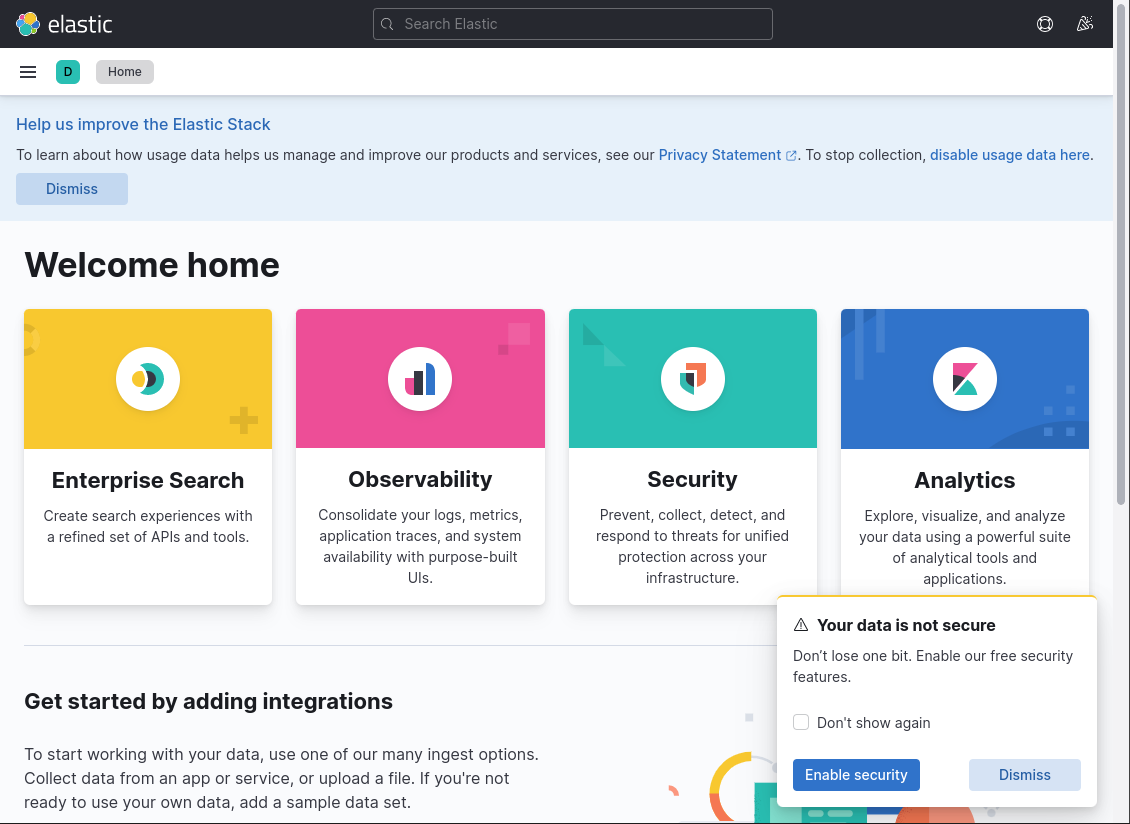
\includegraphics[width=0.8\linewidth]{files/images/kibana-start-page.png}
	\caption{Kibana's start page}
	\label{fig:kibana-start-page}
\end{figure}


\bigskip

From there, it is possible to explore the different Kibana components, import some sample datasets, create Dashboards\dots\ and learn more about Kibana and ElasticSearch in general. \\

\bigskip

For this article, we will only need to use the development tools from Kibana\dots \\

Note: we could use any tool that allows to perform HTTP requests to the ElasticSearch server, but Kibana comes with some extra features as well as auto-completion. \\


\newpage

To access Kibana's Dev Tools, click on the \emph{``hamburger"} menu (top left) >> then scroll down to ``Management" and select ``Dev Tools":


\begin{figure}[h]
	\centering
	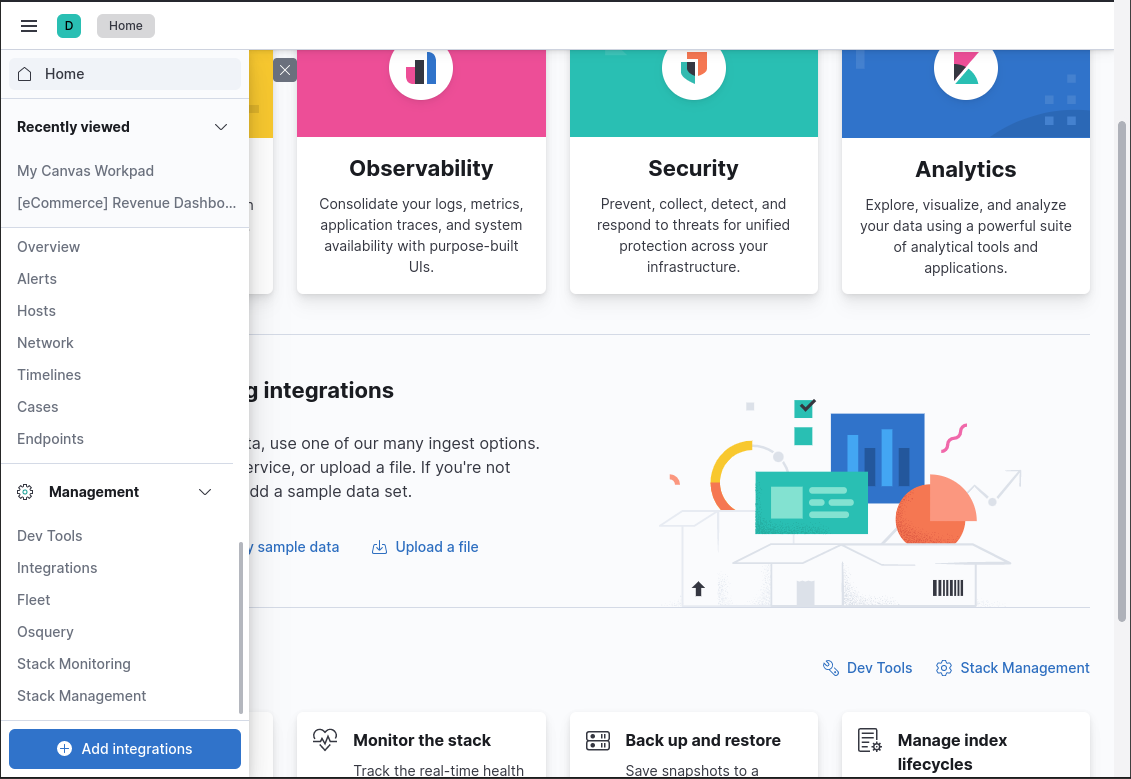
\includegraphics[width=0.8\linewidth]{files/images/kibana-menu}
	\caption{Menu to access Kibana's Dev Tools}
	\label{fig:access-kibana-dev-tools}
\end{figure}

\bigskip

This will lead you to the following screen:

\begin{figure}[h]
	\centering
	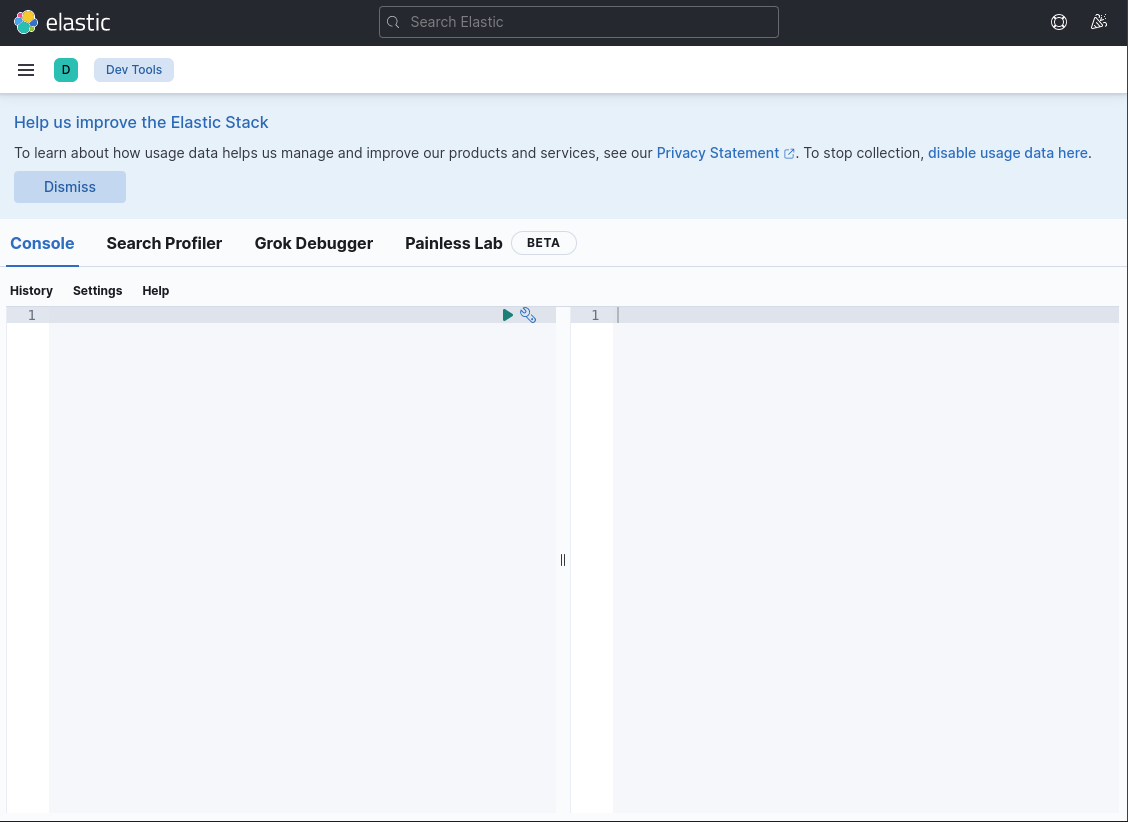
\includegraphics[width=0.8\linewidth]{files/images/kibana-dev-tools}
	\caption{Kibana's Dev Tools}
	\label{fig:kibana-dev-tools}
\end{figure}

\bigskip

On the left side, you can type the HTTP requests to send to ElasticSearch (we will see some examples in section \ref{using-elasticsearch}). The server's responses will be displayed on the right.

\newpage



\section{Using ElasticSearch} \label{using-elasticsearch}

\subsection{Testing that Kuromoji works} \label{es-testing-kuromoji}

The first thing we will do is see if the \kuromoji\ plugin works, by trying to process some text: \\

\begin{lstlisting}[language=sh]
POST _analyze
{
	"tokenizer": "kuromoji_tokenizer",
	"text": """普通の星の下に生まれ 普通の星の下を歩き
	普通の町で 君と出会って 特別な恋をする"""
	,
	"filter": 
	[
 "kuromoji_baseform"
	, "kuromoji_part_of_speech"
	, "cjk_width"
	, "ja_stop"
	, "kuromoji_stemmer"
	, "lowercase"
	]
}
\end{lstlisting}


\bigskip

The result is as follows (edited for brevity):

\begin{lstlisting}[language=sh]
{
	"tokens" : [
	{
		"token" : "普通",
		"start_offset" : 0,
		"end_offset" : 2,
		"type" : "word",
		"position" : 0
	},
	{
		"token" : "星",
		"start_offset" : 3,
		"end_offset" : 4,
		"type" : "word",
		"position" : 2
	},
	{
		"token" : "下",
		"start_offset" : 5,
		"end_offset" : 6,
		"type" : "word",
		"position" : 4
	},
	{
		"token" : "生まれる",
		"start_offset" : 7,
		"end_offset" : 10,
		"type" : "word",
		"position" : 6
	},
	{
		"token" : "普通",
		"start_offset" : 11,
		"end_offset" : 13,
		"type" : "word",
		"position" : 7
	},
	(...)
	]
}
\end{lstlisting}

\bigskip

So as you can see, the \kuromoji\ plugin works. We can also see the result of tokenisation (lexeme, offsets, type, position). \\





\subsection{Creating a core (collection)} \label{create-es-core}

Next, we create a core called \texttt{/song\_jp} : \\

\begin{lstlisting}[language=sh]
PUT /song_jp
{
	"settings": {
		"index": {
			"analysis": {
				"analyzer": {
					"jp_analyser": {
						"tokenizer": "kuromoji_tokenizer",
						"filter": 
						[
						"kuromoji_baseform"
						, "kuromoji_part_of_speech"
						, "cjk_width"
						, "ja_stop"
						, "kuromoji_stemmer"
						, "lowercase"
						]
					}
				}
			}
		}
	}
	,
	"mappings": {
		"dynamic_templates": [
		{
			"txt_japanese": {
				"match_mapping_type": "string",
				"match": "*_txt_ja",
				"mapping": {
					"type": "text",
					"analyzer": "jp_analyser",
					"term_vector": "with_positions_offsets",
					"store" : true,
					"fielddata":true
				}
			}
		}
		,
		{
			"str": {
				"match_mapping_type": "string",
				"match": "*_str",
				"mapping": {
					"type": "keyword"
				}
			}
		}
		]
	}
}
\end{lstlisting}




\bigskip

First we need to configure an analyser for text in Japanese. We need to give it a name: \texttt{jp\_analyser}. 

This analyser will use the \kuromoji\ tokeniser (\texttt{kuromoji\_tokenizer}). \\


\bigskip

\newpage

In Solr, we decided to use dynamic fields (section \ref{dynamic-fields}): 

\begin{itemize}
	\item \texttt{*\_txt\_jp} : fields of Solr type \texttt{text\_ja} (text which is tokenised by \kuromoji, and then indexed and stored)
	
	\item \texttt{*\_str} : fields of Solr type \texttt{strings} (string values that are compared ``as is"; ideal for: tags, categories, etc.)
\end{itemize}

\bigskip

We want to do the same with ElasticSearch:
\begin{itemize}
	\item \texttt{*\_txt\_jp} : fields of ElasticSearch type \texttt{text}, tokenised by \kuromoji, with positions and offsets, stored
	
	\item \texttt{*\_str} : fields of Solr type \texttt{keyword}
\end{itemize}


\bigskip
\bigskip

Finally, the {*\_txt\_jp} fields are declared with \texttt{"fielddata":true}. 

This is necessary to do some \aggregations\ on a field type \texttt{text} (as we will see in section \ref{aggregation-termsVectors}), but it uses more memory. \\

All these fields are defined in \texttt{"dynamic\_templates"}.


\bigskip
\bigskip



\subsection{Deleting a core (collection)}

If at any point you need to delete a core (e.g. to recreated it), perform the following action: \\

\begin{lstlisting}[language=sh]
DELETE /song_jp
\end{lstlisting}

\bigskip



\subsection{Adding a document}

Adding a document is done with the following HTTP request:

\begin{lstlisting}[language=sh]
POST /song_jp/_doc/1
{
	"band_str": "Band name",
	
	"lyrics_txt_ja": 
"""
The song lyrics go there...

(but because of copyright law, 
I cannot give you an actual example)

"""		
}
\end{lstlisting}

\bigskip

The document id is part of the URL (which means it must bne URL-encoded). \\


\bigskip
\bigskip
\bigskip

\subsection{Viewing the \texttt{termsVector}s of a document} \label{es-viewing-termsVector}

\bigskip
To view the \termsVector\ used in every field in the document, you can use the following HTTP request:

\begin{lstlisting}[language=sh]
GET /song_jp/_termvectors/1	
\end{lstlisting}

\bigskip
\dots or if you want the \termsVector\ of one field in particular:

\begin{lstlisting}[language=sh]
GET /song_jp/_termvectors/1?fields=lyrics_txt_ja	
\end{lstlisting}

\bigskip
\dots and you can be precise in your request:

\begin{lstlisting}[language=sh]
GET /song_jp/_termvectors/1?fields=lyrics_txt_ja
{
	"term_statistics": true,
	"field_statistics": true,
	"positions": false,
	"offsets": false,
	"filter": {
		"max_num_terms": 10,
		"min_term_freq": 1,
		"min_doc_freq": 1
	}
}
\end{lstlisting}


\bigskip
\bigskip

These queries allow to inspect the \termsVector s, and the type of information they contain. \\

Result example (edited for brevity):

\begin{lstlisting}[language=sh]
{
	"_index" : "song_jp",
	"_type" : "_doc",
	"_id" : "1",
	"_version" : 1,
	"found" : true,
	"took" : 0,
	"term_vectors" : {
		"lyrics_txt_ja" : {
			"field_statistics" : {
				"sum_doc_freq" : 130,
				"doc_count" : 3,
				"sum_ttf" : 276
			},
			"terms" : {
				"いける" : {
					"term_freq" : 1,
					"tokens" : [
					{
						"position" : 6,
						"start_offset" : 12,
						"end_offset" : 14
					}
					]
				},
				(...)
			
			        "愛する" : {
				"term_freq" : 4,
				"tokens" : [
				{
					"position" : 108,
					"start_offset" : 208,
					"end_offset" : 211
				},
				{
					"position" : 193,
					"start_offset" : 353,
					"end_offset" : 356
				},
				{
					"position" : 199,
					"start_offset" : 363,
					"end_offset" : 366
				},
				{
					"position" : 205,
					"start_offset" : 373,
					"end_offset" : 376
				}
				]
			},
			(...)
		}
	}
}
\end{lstlisting}



\bigskip
\bigskip
\bigskip



\subsection{Aggregation on \texttt{termsVectors}} \label{aggregation-termsVectors}

Now we reach the part where we want to answer questions of the type: \emph{``Which words are the most used in (a certain result-set) ?"} \\

As we have seen many times in section \emph{\longref{exploring-dataset}}, this is done with an aggregation on a text field containing \termsVector s (and \texttt{fielddata}). \\

\begin{lstlisting}[language=sh]
GET /song_jp/_search
{
	"size": 0,
	"aggs": {
		"test": {
			"terms": {
				"field": "lyrics_txt_ja",
				"size": 100
			}
		}
	}
}
\end{lstlisting}

This query is only possible if the field used in the \faceting\ has been declared with \texttt{"fielddata": true} . \\

If the \texttt{"fielddata"} was not set, then we would be met with the following error:

\begin{lstlisting}[language=sh]
“Fielddata is disabled on text fields by default. Set `fielddata=true` on [`your_field_name`] in order to load field data in memory by uninverting the inverted index. Note that this can however, use “significant memory.” – if this happens you can either enable the field-data on that text field, or choose another way to query the data (again, because field-data consumes a lot of memory and is not recommended).
\end{lstlisting}

\bigskip
\bigskip

We are more interested in the result of the aggregation (list of terms) than the list of documents. So we set the \texttt{size} of the result-set (list of documents) to 0. \\

Then we specify the \texttt{size} of the aggregation to the number of terms we want to display (default value: 10). \\


\bigskip
\bigskip
\bigskip

The result looks something like this:

\begin{lstlisting}[language=sh]
{
	"took" : 24,
	"timed_out" : false,
	"_shards" : {
		"total" : 1,
		"successful" : 1,
		"skipped" : 0,
		"failed" : 0
	},
	"hits" : {
		"total" : {
			"value" : 3,
			"relation" : "eq"
		},
		"max_score" : null,
		"hits" : [ ]
	},
	"aggregations" : {
		"test" : {
			"doc_count_error_upper_bound" : 0,
			"sum_other_doc_count" : 109,
			"buckets" : [
			{
				"key" : "時",
				"doc_count" : 3
			},
			{
				"key" : "何",
				"doc_count" : 2
			},
			{
				"key" : "僕",
				"doc_count" : 2
			},
			{
				"key" : "君",
				"doc_count" : 2
			},
			(...)
			
			]
		}
	}
}
\end{lstlisting}


\bigskip
\bigskip


%\newpage

\subsection{ElasticSearch's ``More Like This"}

We have talked about the \MLT\ queries, and show how to run them in Solr in section \emph{\longref{mlt}}. \\


Performing a \MLT\ query in ElasticSearch is easy. Here is an example with one document:

\newpage

\begin{lstlisting}[language=sh]
GET /_search
{
	"query": {
		"more_like_this": {
			"fields": [ "lyrics_txt_ja" ],
			"like": [
			{
				"_index": "song_jp",
				"_id": "1"
			}        
			],
			"min_term_freq": 1,
			"max_query_terms": 12
		}
	}
}
\end{lstlisting}

\bigskip


It is also possible to perform a \MLT\ query on more than one document, and also one custom text:

\begin{lstlisting}[language=sh]
GET /_search
{
	"query": {
		"more_like_this": {
			"fields": [ "lyrics_txt_ja" ],
			"like": [
			{
				"_index": "song_jp",
				"_id": "1"
			}        
			],
			{
				"_index": "song_jp",
				"_id": "2"
			},
			"You can also perform a 'More Like This' query on custom text, not just on documents."
			],
			"min_term_freq": 1,
			"max_query_terms": 12
		}
	}
}
\end{lstlisting}

\bigskip

A notable difference with Solr: in ElasticSearch, you can pass a list of documents or custom strings on which to run the \MLT\ query, whereas in Solr you pass a query (which may return one or more documents) and the \MLT\ feature is run on the result of this query (as shown in section \ref{mlt-solr-example}). \\

On one hand, Solr allows you to run \MLT\ on the result of a query. On the other hand,  ElasticSearch allows you to run \MLT\ on a custom query. \\

In practice though, you would rarely want to run a \MLT\ query on more than one document (because the results become less relevant). Being able to run \MLT\ on a custom string can be convenient. \\



\url{https://www.elastic.co/guide/en/elasticsearch/reference/current/query-dsl-mlt-query.html}







\newpage
% Copyright 2022 Pierre S. Caboche. All rights reserved.

\renewcommand{\currentPart}{Final words}
\part{\currentPart} \label{part - Final words}


\section{Comparing Solr and ElasticSearch}


\begin{itemize}
	\item \emph{Solr is easier to get started with}
\end{itemize}

Getting Solr started was easy: one \texttt{docker run} command and the latest image was downloaded, the container created, and Solr was up and running (for testing purposes). All the results you see in this document were gathered on Solr. \\ 

Then I tried to replicate our study in the immensely popular ElasticSearch\dots \\


\bigskip
	
I wanted to run ElasticSearch with Kibana. Although not strictly necessary, Kibana provides ways to interact with ElasticSearch other than through a web API. I wanted to evaluate the UI, and compare it to what Solr provides out-of-the-box. \\

I read the official documentation for ElasticSearch (currently at version 8.3.3), created the \texttt{docker-compose} files as instructed (for ElasticSearch and Kibana), tried to execute them, and was greeted with the following message (for all versions from 8.3.1 to 8.3.3):
\begin{lstlisting}
ERROR: for kibana  Container "............" is unhealthy.
ERROR: Encountered errors while bringing up the project.
\end{lstlisting}


\bigskip

Version 7.17.5 was easier to get to work. \\

Unlike with Solr, the \kuromoji\ plugin was not installed by default. This meant writing a \texttt{Dockerfile} to create a custom image, and a \texttt{docker-compose.yml} to run the custom image in a container (with all the parameters that we need). \\

As you can see, the process was more complicated, and I didn't get to run the latest version despite following the documentation to the letter. \\

I hope this would be fixed in the future\dots \\


\bigskip


\begin{itemize}
	\item \emph{ElasticSearch has more features} 
\end{itemize}

ElasticSearch in itself has more features, and those features tend to be more advanced. On top of that, there is a whole environment around ElasticSearch: Kibana (for visualisation), and Logstash (for data integration). \\

ElasticSearch offers some really advanced \aggregations, while Solr only provides basic \faceting. \\

Kibana allows to visualise, explore data, create dashboards, and many other things with the appropriate licence (e.g. Machine Learning). \\

A clear win for ElasticSearch. \\

\bigskip
\bigskip

\begin{itemize}
	\item \emph{Solr is free}
\end{itemize}

Solr is free (it is under Apache License 2.0) \\

ElasticSearch has a dual-licence (both proprietary; source-available): the Elastic License, and the Server Side Public License. \\





\section{Conclusion}

This article started as a way to teach the basics of Solr, ElasticSearch, indexing for full-text search, \faceting\ / \aggregations\ (for which we found some interesting use). Then to illustrate how those principles work, we created a catalogue of songs which we wanted to query in different manners. \\

This led us to analyse the lyrics of Japanese songs, by running different statistics about word usage (most used words overall, most used words for a particular band or songwriter, list of bands using a certain word the most\dots) \\

From a technical point of view, we have learned a number of things:
\begin{itemize}
	\item fields, types, dynamic fields
	\item termsVectors, indexing different languages
	\item \faceting, \aggregations, \MLT\ features
	\item some of the differences between Solr and ElasticSearch %(both based on Apache Lucene)
\end{itemize}

We tried to give just enough information to understand the main concepts and become operational quickly. Exploring the dataset (which we created to show the tool's capabilities) would constitute the bulk of this paper. \\

The tool that we created (a set of scripts to interact with Solr) allow us to run statistics, and find commonalities between songs from different bands, and across genres. 
Starting with a list of common words (sections~\ref{general-queries} to~\ref{most-used-words-by-songwriter}), we can determine the likelihood of a given band to use a certain word (section~\ref{word-usage}), thereby allowing us to establish some sort of profile for certain bands, songwriters, etc. \\

This idea is taken a step further with the \MLT\ feature (section~\ref{mlt}). Given one document (song), it is capable to find a list of documents featuring similar terms (based on \emph{term frequency–inverse document frequency}, section~\ref{tf–idf}). The connections it makes is sometimes very surprising (but all based on statistics), and it can help you discover songs with similar lyrics to the ones you already like. \\

As we add more songs to the dataset, find new ``interesting terms" to explore and run statistics on, we get more insights on the bands' writing styles, and the type of lexicon used in a popular art form. \\

The data presented in \emph{``section \longref{exploring-dataset}"} are only a fraction of the results we gathered. We can establish more statistics by band or lexemes, more suggestions with the \MLT\ feature.
The only thing I cannot do is share the dataset, for legal reasons.
\\






\renewcommand{\formatPartTitle}{}





\listoffigures



% Label on the last page. Allows to easily get the page number
\label{LastPage}

\end{document}
